%# -*- coding:utf-8 -*-
\chapter{数值仿真与实验结果分析}\label{chap:exp}
\echapter{Numerical Simulations and Analysis}

本章将通过大量的实验来展示本文所提出方法的优越性及特点。首先介绍实验的相关设置,而后给出实验结果并加以分析。

\section{实验设置}
\esection{Experimental Setups}
本节将分别介绍无监督特征选择与提取任务下的数据集、评价指标与方法、对比方法以及参数设置。在本文中,所有的程序均通过MATLAB R2020b编写。此外,所有的实验均运行在一台配备3.70-GHZ i9-10900K CPU和128-GB主内存的Ubuntu服务器上,并且没有使用GPU。当需要在MATLAB中操作张量时,本文使用MATLAB张量工具箱\footnote{\url{https://www.tensortoolbox.org/}}来进行处理。
% 此外,当我们需要使用求解器来求解二阶锥规划时,我们使用业内领先的求解器MOSEK\ucite{mosek}。

\subsection{无监督特征选择实验设置}\label{sec:expsetup-ufs}
\esubsection{Experimental Setups for Unsupervised Feature Selection}
首先介绍使用到的数据集。本文采用了十个真实世界基准数据集,包括两个目标检测数据集(FashionMNIST\footnote{\url{https://github.com/zalandoresearch/fashion-mnist}}和COIL20\footnote{\label{foot:dengcai}\url{http://www.cad.zju.edu.cn/home/dengcai/Data/data.html}}),五个人脸识别数据集(ORL\,\textsuperscript{\ref{foot:dengcai}}、UMIST\footnote{\label{foot:umist}\url{https://eprints.lincoln.ac.uk/id/eprint/16081/}}、Pixraw10P\footnote{\label{foot:jundongl}\url{https://jundongl.github.io/scikit-feature/datasets.html}}、Orlraws10P\,\textsuperscript{\ref{foot:jundongl}}和JAFFE\footnote{\url{https://zenodo.org/record/3451524}}),以及三个医学图像分类数据集(BreastMNIST\footnote{\label{foot:medmnist}\url{https://medmnist.com/}}、OCTMNIST\,\textsuperscript{\ref{foot:medmnist}}和OrganSMNIST\,\textsuperscript{\ref{foot:medmnist}})。作为预处理,上述数据集中的每幅图像的值均被归一化至$[0,1]$。由于在本任务中没有区分训练集与测试集,因而不需要对数据集进行进一步的划分。这些数据集的统计信息如\reftab{tab:datesets-ufs}所示。

\begin{table}[!t]
\centering
\caption{十个用于无监督特征选择的真实世界基准数据集的统计信息}
\label{tab:datesets-ufs}
\begin{tabular}{lrrrr}
\toprule
数据集名称 & 样本数 & 特征尺寸 & 类别数 & 被选择的特征数量区间 \\ \midrule
FashionMNIST  & $1$,$000$          & $28$ $\times$ $28$         & $10$            & $[50,100,150,\ldots,300]$            \\
COIL20  & $1$,$440$          & $32$ $\times$ $32$         & $20$            & $[50,100,150,\ldots,300]$            \\
ORL  & $400$          & $32$ $\times$ $32$         & $40$            & $[50,100,150,\ldots,300]$            \\
UMIST  & $575$          & $23$ $\times$ $28$         & $20$            & $[50,100,150,\ldots,300]$            \\
Pixraw10P     & $100$           & $100$ $\times$ $100$         & $10$            & $[50,100,150,\ldots,300]$             \\
Orlraws10P    & $100$           & $92$ $\times$ $112$         & $10$            & $[50,100,150,\ldots,300]$            \\
BreastMNIST  & $288$          & $28$ $\times$ $28$         & $2$            & $[50,100,150,\ldots,300]$            \\
OCTMNIST      & $400$          & $28$ $\times$ $28$         & $4$            & $[50,100,150,\ldots,300]$  \\
OrganSMNIST    & $220$          & $28$ $\times$ $28$         & $11$            & $[50,100,150,\ldots,300]$            \\
JAFFE    & $213$          & $64$ $\times$ $64$         & $10$            & $[50,100,150,\ldots,300]$            \\
\bottomrule
\end{tabular}

\end{table}

接下来介绍评价指标与方法。在本任务中,由于没有区分训练集与测试集,因而直接在整个数据集上应用不同的方法来选择特征。在特征选择完成之后,通过在被选择特征上的$k$-means聚类\ucite{李航2012统计学习方法}性能来评估被选择特征的质量。本文采用两种被广泛使用的评价指标归一化的互信息(Normalized Mutual Information, NMI)和准确率(Accuracy, ACC)\ucite{cai2010graph}来评估$k$-means聚类的性能。NMI与ACC越高,代表$k$-means聚类的性能越好,因而表示被选择特征的质量越高,也就代表特征选择方法的性能越强。由于$k$-means聚类的结果部分取决于其初始化,因而采用以下策略来缓解评价系统中内在的随机性:对于任意一组被选择的特征,将$k$-means聚类重复运行$20$次并记录平均结果及标准差。

设$n$为样本的总数,$l_i$为第$i$个样本的真实标签,$r_i$为第$i$个样本的聚类标签,并令$\boldsymbol{l}=[l_{1},l_{2},\ldots,l_{n}]$,$\boldsymbol{r}=[r_{1},r_{2},\ldots,r_{n}]$,则NMI与ACC的定义如下
\begin{equation*}
\text{NMI}(\boldsymbol{l}, \boldsymbol{r})=\frac{\operatorname{I}(\boldsymbol{l}, \boldsymbol{r})}{\sqrt{\operatorname{H}(\boldsymbol{l}) \operatorname{H}(\boldsymbol{r})}},
\end{equation*}
\begin{equation*}
    \text {ACC}(\boldsymbol{l}, \boldsymbol{r}) = \frac {1} { n } \sum _ { i = 1 } ^ { n } \delta \left( l _ { i }, \operatorname { map } \left( r _ { i } \right) \right) ,
\end{equation*}
其中$\operatorname{I}(\boldsymbol{l},\boldsymbol{r})$、$\operatorname{H}(\boldsymbol{l})$以及$\operatorname{H}(\boldsymbol{r})$分别为$\boldsymbol{l}$与$\boldsymbol{r}$之间的互信息以及$\boldsymbol{l}$与$\boldsymbol{r}$各自的边际熵\ucite{cover1999elements},而$\operatorname{map}(\cdot)$则为基于匈牙利算法\ucite{kuhn1955hungarian}的最佳排列映射。

最后介绍对比方法与参数设置。为了验证CPUFS与CPUFSnn方法的有效性\footnote{CPUFS与CPUFSnn方法已开源于\url{https://github.com/Kwan1997/CPUFS}},本文将它们与九种前沿的无监督特征选择方法进行比较
% \footnote{本文不会与GRLTR这一基于张量优化的无监督特征选择方法对比,因为它是一种嵌入式特征选择方法,而这超出了本文的范围(本文关注于过滤式特征选择)。}
,包括LapScore\ucite{lapscore}、MCFS\ucite{cai2010unsupervised}、UDFS\ucite{udfs}、SOCFS\ucite{socfs}、SOGFS\ucite{sogfs}、RUFS\ucite{rufs}、RSFS\ucite{rsfs}、 JELSR\ucite{jelsr}以及CDLFS\ucite{cdlfs}。这些方法的详细描述可以在\refsection{sec:review-ufs}中找到。SOGFS的代码由本文作者自行编写实现,而其它所有方法的代码均由其作者提供。此外,还采用仅选择所有原始特征的基线方法AllFea来说明特征选择的效用性所在。本文通过网格搜索策略在$\{10^{-2},10^{-1},1,\allowbreak 10,\allowbreak 10^{2}\}$内调整所有方法的参数。对于CPUFS方法,在所有数据集上均设置$\eta=10^{5}$;对于CPUFSnn方法,在OCTMNIST以及OrganSMNIST数据集上设置$\eta=10^{4}$,而在除这两个数据集以外的所有数据集上均设置$\eta=10^{5}$。对于使用到加权$k$近邻图的方法,设置近邻的数量$k=5$以及高斯核宽度$\sigma=1$。对于基于投影的方法,将投影子空间的维度设置为数据中的类别数的真值$c$;对于基于聚类的方法,也将潜在类别的数量设置为数据中的类别数的真值$c$。此外,设置$\Phi_{1}=500$和$\Phi_{2}=2$。对于每种不同的方法,本文展示其在所有参数组合下的最佳效果。


\subsection{无监督特征提取实验设置}\label{sec:expsetup-ufe}
\esubsection{Experimental Setups for Unsupervised Feature Extraction}

\begin{table}[!t]
	\caption{三个用于无监督特征提取的真实世界基准数据集的统计信息}
	\label{tab:datesets-ufe}
	\centering
% 	\begin{tabular}{lrrr}
% \toprule
% 数据集名称              & COIL20           & Yale           & UMIST          \\ \midrule
% 样本数              & 1,440           & 165            & 565            \\
% 特征尺寸           & $32 \times 32$ & $32 \times 32$ & $32 \times 32$ \\
% 类别数              & 20             & 15             & 20             \\
% 训练集规模 & $32 \times 32 \times 160$ & $32 \times 32 \times 120$ & $32 \times 32 \times 150$ \\
% 测试集规模     & $32 \times 32 \times 1,280$ & $32 \times 32 \times 45$ & $32 \times 32 \times 415$ \\ \bottomrule
% \end{tabular}%
\begin{tabular}{@{}lrrrrr@{}}
\toprule
数据集名称  & 样本数   & 特征尺寸           & 类别数 & 训练集规模                     & 测试集规模                       \\ \midrule
COIL20 & 1,440 & $32 \times 32$ & 20  & $32 \times 32 \times 160$ & $32 \times 32 \times 1,280$ \\
Yale   & 165   & $32 \times 32$ & 15  & $32 \times 32 \times 120$ & $32 \times 32 \times 45$    \\
UMIST  & 565   & $32 \times 32$ & 20  & $32 \times 32 \times 150$ & $32 \times 32 \times 415$   \\ \bottomrule
\end{tabular}%

\end{table}

首先介绍使用到的数据集。本文采用了三个真实世界基准数据集,包括一个目标检测数据集(COIL20\,\textsuperscript{\ref{foot:dengcai}}),两个人脸识别数据集(Yale\,\textsuperscript{\ref{foot:dengcai}}以及UMIST\,\textsuperscript{\ref{foot:umist}})。作为预处理,上述数据集中的每幅图像均被下采样至$32 \times 32$,并且它们的值均被归一化至$[0,1]$。由于在本任务中区分了训练集与测试集,因此需要对数据集进行进一步的划分。这些数据集的具体划分结果以及它们的统计信息如\reftab{tab:datesets-ufe}所示。此外,由于$\ell_{1}$与$\ell_{\infty}$方法旨在抑制数据中的噪声与离群点所带来的负面影响,因而本节还为这三个数据集设计了大量的噪声场景。首先介绍这些噪声的类型。具体而言,为COIL20数据集设计了四种类型的噪声:
\begin{enumerate}
    \item {\boldmath\bfseries ms-$n_{1}\text{-}n_{2}\text{-}n_{3}$:}在训练集的每八张图片中,前三张分别有$n_{1}\%$、$n_{2}\%$以及$n_{3}\%$的像素被随机移除;
    \item {\boldmath\bfseries ms-$n_{1}\text{-}n_{2}\text{-}n_{3}\text{-}n_{4}$:}在训练集的每八张图片中,前四张分别有$n_{1}\%$、$n_{2}\%$、$n_{3}\%$以及$n_{4}\%$的像素被随机移除;
    \item {\boldmath\bfseries sp-$n_{1}\text{-}n_{2}\text{-}n_{3}$:}在训练集的每八张图片中,前三张分别受到密度为$n_{1}\%$、$n_{2}\%$以及$n_{3}\%$的椒盐型噪声污染;
    \item {\boldmath\bfseries sp-$n_{1}\text{-}n_{2}\text{-}n_{3}\text{-}n_{4}$:}在训练集的每八张图片中,前四张分别受到密度为$n_{1}\%$、$n_{2}\%$、$n_{3}\%$以及$n_{4}\%$的椒盐型噪声污染。
\end{enumerate}
为Yale数据集设计了两种类型的噪声:
\begin{enumerate}
    \item {\boldmath\bfseries ms-$n_{1}\text{-}n_{2}\text{-}n_{3}$:}在训练集的每八张图片中,前六张分别有$n_{1}\%$、$n_{1}\%$、$n_{2}\%$、$n_{2}\%$、$n_{3}\%$以及$n_{3}\%$的像素被随机移除;
    \item {\boldmath\bfseries sp-$n_{1}\text{-}n_{2}\text{-}n_{3}$:}在训练集的每八张图片中,前六张分别分别受到密度为$n_{1}\%$、$n_{1}\%$、$n_{2}\%$、$n_{2}\%$、$n_{3}\%$以及$n_{3}\%$的椒盐型噪声污染。
\end{enumerate}
为UMIST数据集设计了两种类型的噪声:
\begin{enumerate}
    \item {\boldmath\bfseries ms-$n_{1}\text{-}n_{2}\text{-}n_{3}$:}在训练集中被随机选择的45张图像中,分别有25、15以及5张图像各自有$n_{1}\%$、$n_{2}\%$以及$n_{3}\%$的像素被随机移除;
    \item {\boldmath\bfseries sp-$n_{1}\text{-}n_{2}\text{-}n_{3}$:}在训练集中被随机选择的45张图像中,分别有25、15以及5张图像分别受到密度为$n_{1}\%$、$n_{2}\%$以及$n_{3}\%$的椒盐型噪声污染。
\end{enumerate}
基于如上设计的噪声类型,生成了如下的噪声场景:
\begin{enumerate}
    \item 在COIL20数据集上,一共生成了34种噪声场景,如\reftab{tab:coil}所示;
    % as shown in \reffig{fig:corr-coil},
    \item 在Yale数据集上,一共生成了18种噪声场景,如\reftab{tab:yale}所示;
    % as shown in \reffig{fig:corr-yale}.
    \item 在UMIST数据集上,一共生成了18种噪声场景,如\reftab{tab:umist}所示。
    % as shown in \reffig{fig:corr-umist}, and
\end{enumerate}
% 本文在附录\refsection{sec:noise-comp}中给出了每一种生成的噪声的示例,以供读者有一个直观的认识。这些生成的噪声图像将用于随后的实验中。

接下来介绍评价指标与方法。由于在本任务中区分了训练集与测试集,因而首先在训练集中应用不同的方法学习得到特征提取器(例如在$\ell_{\infty}$方法中即为$\{\boldsymbol{A}^{(j)}\}_{j=1}^{d}$),而后在测试集上应用学习得到的特征提取器进行特征提取。在特征提取完成之后,通过在被提取特征上的$k$近邻($k$-Nearest Neighbour, KNN)分类性能以及支持向量机(Support Vector Machine, SVM)分类性能来评估被提取特征的质量。本文采用被广泛使用的评价指标ACC\ucite{cai2010graph}来评估分类的性能。(此处的ACC与无监督特征选择任务中的ACC是基本一致的。唯一不同之处在于,由于在本任务中采用分类策略来评估特征提取的质量,因而不再需要匈牙利算法来实现最佳排列(或认为$\operatorname{map}(\cdot)$=$\operatorname{id}(\cdot)$,恒同映射)。故此处不再赘述其具体数学表达式。)ACC越高,代表分类器的性能越好,因而表示被提取特征的质量越高,也就代表特征提取方法的性能越强。

最后介绍对比方法与参数设置。为了验证$\ell_{1}$与$\ell_{\infty}$方法的有效性\footnote{$\ell_{1}$与$\ell_{\infty}$方法已开源于\url{https://github.com/Kwan1997/Linf}},本文将其与$\ell_{2}$方法以及其它六种经典的无监督特征提取方法进行比较,包括概率主成分分析方法(Probabilistic PCA, ProbPCA)\ucite{ProbPCA}、因子分析方法(Factor Analysis, FA)\ucite{FA}、保距映射方法(Isometric Mapping, IsoMap)\ucite{IsoMap}、局部线性嵌入方法(Locally Linear Embedding, LLE)\ucite{LLE}、拉普拉斯特征图方法(Laplacian Eigenmaps, LapE)\ucite{LapE} 以及自编码器方法(Autoencoder, AE)\ucite{Goodfellow2016}。对于这六种经典无监督特征提取方法,它们的代码均由Matlab降维工具箱\footnote{\url{https://lvdmaaten.github.io/drtoolbox/}}提供。此外,由于这六种经典方法是基于矩阵优化的,因而在应用它们时会将数据向量化。由于$\ell_{1}$、$\ell_{2}$以及$\ell_{\infty}$方法并没有内置参数,因此无需对其进行参数调整。对于IsoMap、LLE和LapE,设置其$k$近邻图的$k=20$。此外,由于这三种方法不支持精确的样本外映射,故使用了Nystr{\"o}m逼近算法\ucite{farahat2011novel}来从测试集中提取特征。对于AE,将其全连接层尺寸设置为$f_{0}\shortrightarrow \ceil{1.2f_{0}}+5\shortrightarrow \ceil{f_{0}/4}+3\shortrightarrow \ceil{f_{0}/10}\shortrightarrow f$,其中$f_{0}$表示原始特征的数量(在本文中,对于所有数据集而言均为$32\times 32=1,024$),而$\ceil{\cdot}$是向上取整函数。此外,通过三折交叉验证以及参数网格搜索策略来调整两个分类器的参数。具体来讲,在搜索空间$\{1,2,\ldots,10\}$中为$k$近邻分类器的$k$参数进行调整,以及在搜索空间$\{2^{i}\}_{i=-7}^{7}$中为支持向量机分类器的两个参数进行调整。对于每种不同的方法,本文展示其在所有参数组合下的最佳效果。
% 它的定义为
% \begin{equation*}
%     \ceil{x}=\min \{n \in \mathbb{Z} \mid n \geq x\}.
% \end{equation*}


% \subsection{实验环境设置与数据集介绍}\label{sec:dataset}
% \esubsection{Environmental Settings and Dataset Introduction}

% % \subsection{数据集}\label{sec:dataset}
% % \esubsection{Datasets}

% \subsection{评价指标与评价方法}
% \esubsection{Evaluation Metrics and Evaluation Methodology}

% \subsection{对比方法与参数设置}\label{sec:comp-methods}
% \esubsection{Comparative Methods and Parameter Settings}

\section{无监督特征选择实验}
\esection{Experiments on Unsupervised Feature Selection}
本节将展示无监督特征选择任务的实验结果,并加以分析。
\begin{sidewaysfigure}
    \centering
    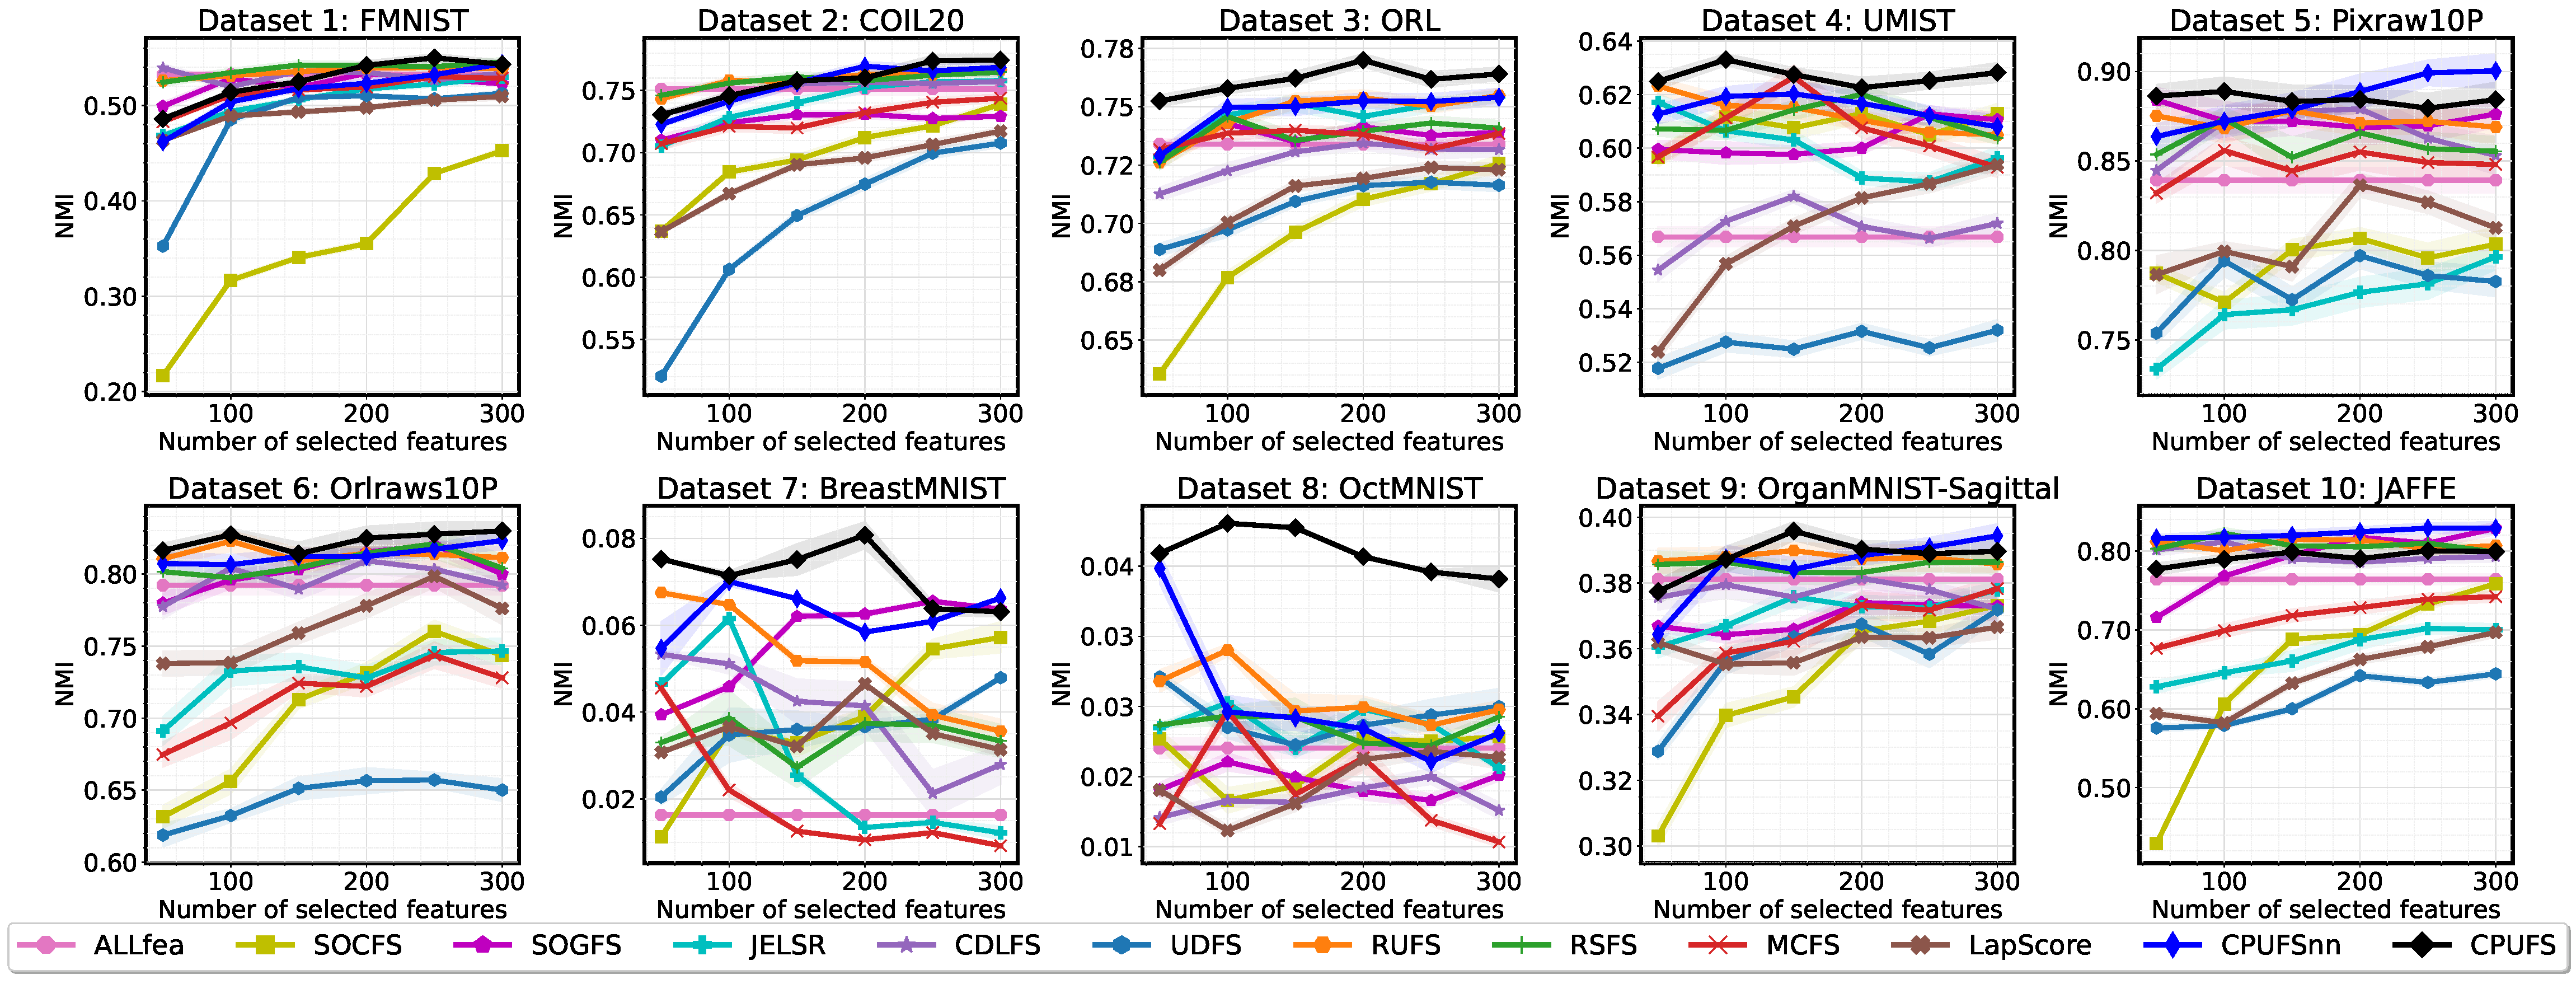
\includegraphics[width=\linewidth]{figures/CPUFS/NMIACC/PAMI_NMI.pdf}
    \caption{不同的无监督特征选择方法在十个数据集上的NMI效果对比}
    \label{fig:clusnmi}
\end{sidewaysfigure}

\begin{sidewaysfigure}
    \centering
    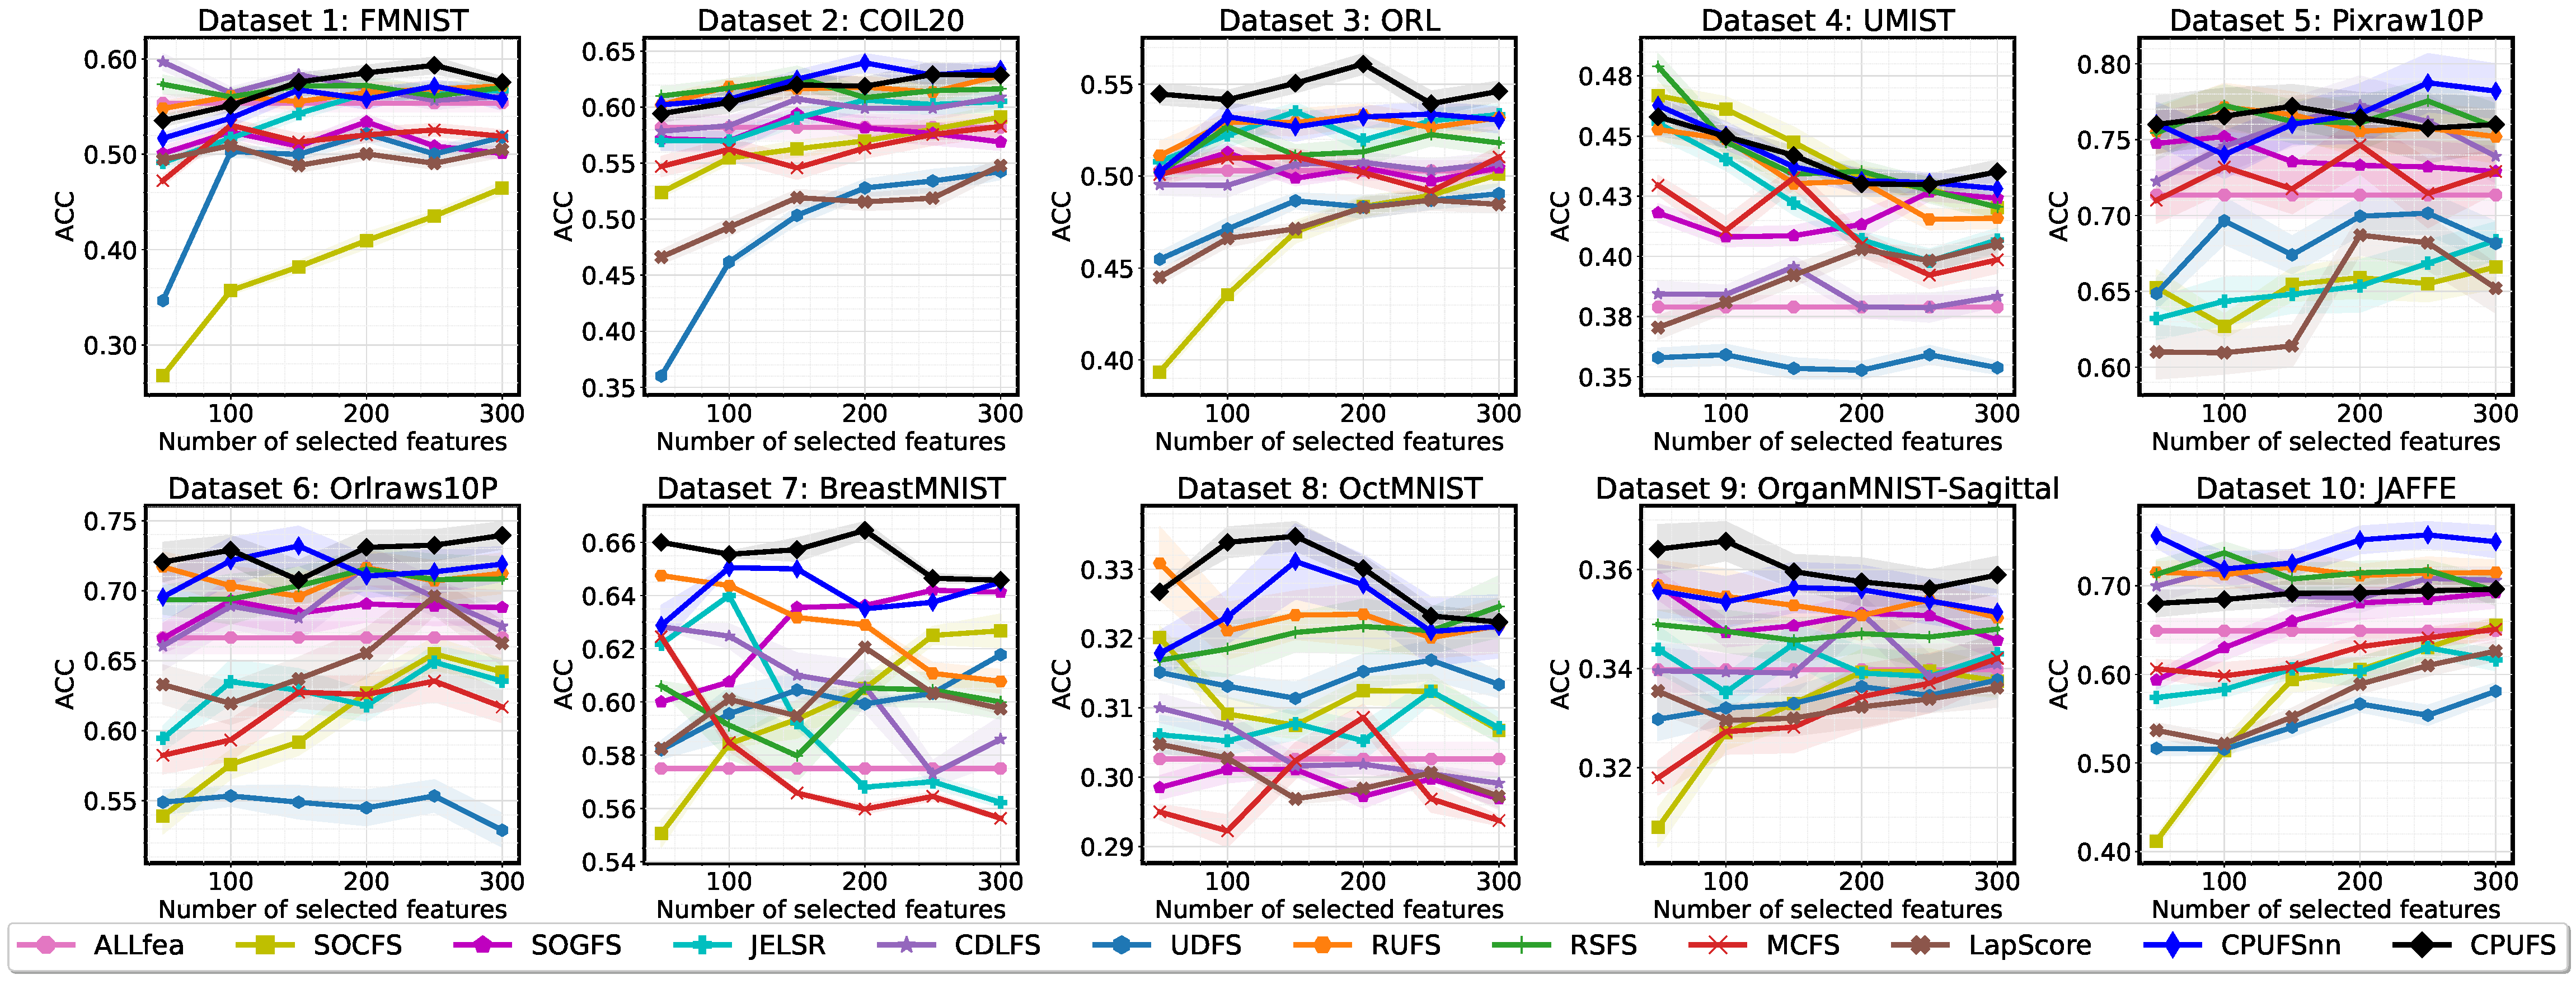
\includegraphics[width=\linewidth]{figures/CPUFS/NMIACC/PAMI_ACC.pdf}
    \caption{不同的无监督特征选择方法在十个数据集上的ACC效果对比}
    \label{fig:clusacc}
\end{sidewaysfigure}

% \subsection{实验一:CPUFS与CPUFSnn和前沿无监督特征选择方法的性能对比}
% \esubsection{Experiment 1: Performance Comparison of the CPUFS and CPUFSnn Methods against the State-of-the-Arts}
\subsection{性能对比}
\esubsection{Performance Comparison}
本节通过比较在被选择特征上的聚类性能来评估不同无监督特征选择方法的性能。
具体来讲,首先分别使用不同的无监督特征选择方法在\refsection{sec:expsetup-ufs}中所提及的所有数据集中进行特征选择,然后基于被选择的特征使用$k$-means聚类算法进行聚类,并依据聚类互信息与准确率来评估不同特征选择方法的性能。
实验结果如\reffig{fig:clusnmi}和\reffig{fig:clusacc}所示,其中阴影区域代表区间$[\mu-0.2\sigma,\mu+0.2\sigma]$(其中$\mu$和$\sigma$分别代表$20$次$k$-means聚类实验的平均值和标准差)。为了方便凸显本文提出的方法,使用具有更大菱形标记的黑色折线代表CPUFS方法,而使用具有较小菱形标记的深蓝色折线代表CPUFSnn方法。基于\reffig{fig:clusnmi}和\reffig{fig:clusacc},可以得出以下结论:
\begin{enumerate}
    \item \textbf{特征选择可提高数据质量:}
    与基线方法ALLfea相比,几乎所有无监督特征选择方法均具有更强的$k$-means聚类性能。这表明特征选择确实可以过滤数据中的冗余和嘈杂特征,因此具有非常重要的作用。
    \item \textbf{CPUFS和CPUFSnn方法在性能上超过了前沿方法:}
    就可达到的最大NMI而言,在这十个数据集之中的任意一个上,总有CPUFS与CPUFSnn中的一个方法是最优的,并且有时CPUFS与CPUFSnn同时包揽前二。虽然在最大可达的ACC方面,CPUFS与CPUFSnn方法并不总是最好的,但在除了FashionMNIST和UMIST之外的所有数据集上,它们之中至少有一个方法仍然可以优于所有对比方法。这充分说明了CPUFS和CPUFSnn方法的有效性。
    % 这主要归因于CPUFS和CPUFSnn方法完好地保留了张量的结构信息。
    \item \textbf{CPUFS和CPUFSnn方法分别适用于不同的场合:}从\reffig{fig:clusnmi}和\reffig{fig:clusacc}中不难发现,其实很难确定究竟是CPUFS方法更好还是CPUFSnn方法更好。例如,在JAFFE数据集上,CPUFSnn方法会达到比CPUFS方法更好的性能;而在ORL数据集上,CPUFSnn方法却表现地比CPUFS方法更差。这个现象表明,线性分类器的非负性并不总是有利于特征选择,但在某些情况下,它确实提升了被选择特征的质量。因此需要因地制宜地确定是否该对线性分类器施加非负约束。
    \item \textbf{“天下没有免费的午餐”\ucite{wolpert1997no}:}可以从\reffig{fig:clusnmi}和\reffig{fig:clusacc}中观察到,没有一种无监督特征选择方法可以在所有数据集上均达到最优,并且不同的方法最适用于不同的数据集。 例如,就ACC而言,SOCFS在FashionMNIST数据集上表现地最差,然而在UMIST数据集上,它又表现地相当之好。尽管如此,值得注意的是,CPUFS和CPUFSnn方法可以较为稳定地在几乎所有数据集上就所有评价指标而言均有优秀的性能。这凸显了它们的稳健性和有效性。
\end{enumerate}

\begin{figure}[!t]
    \centering
    % \subfloat[null]{
\includegraphics[width=0.33\linewidth]{figures/CPUFS/visualization/feaOriginal_ORL.pdf}}
    % \subfloat[null]{
\includegraphics[width=0.33\linewidth]{figures/CPUFS/visualization/feaOriginal_ORL.pdf}}
    % \subfloat[null]{
\includegraphics[width=0.33\linewidth]{figures/CPUFS/visualization/feaOriginal_ORL.pdf}}\\
    % \subfloat[null]{
\includegraphics[width=0.33\linewidth]{figures/CPUFS/visualization/feaOriginal_ORL.pdf}}
    % \subfloat[null]{
\includegraphics[width=0.33\linewidth]{figures/CPUFS/visualization/feaOriginal_ORL.pdf}}
    % \subfloat[null]{
\includegraphics[width=0.33\linewidth]{figures/CPUFS/visualization/feaOriginal_ORL.pdf}}
    \subfloat[FashionMNIST ($\nu$)\label{fig:f1}] {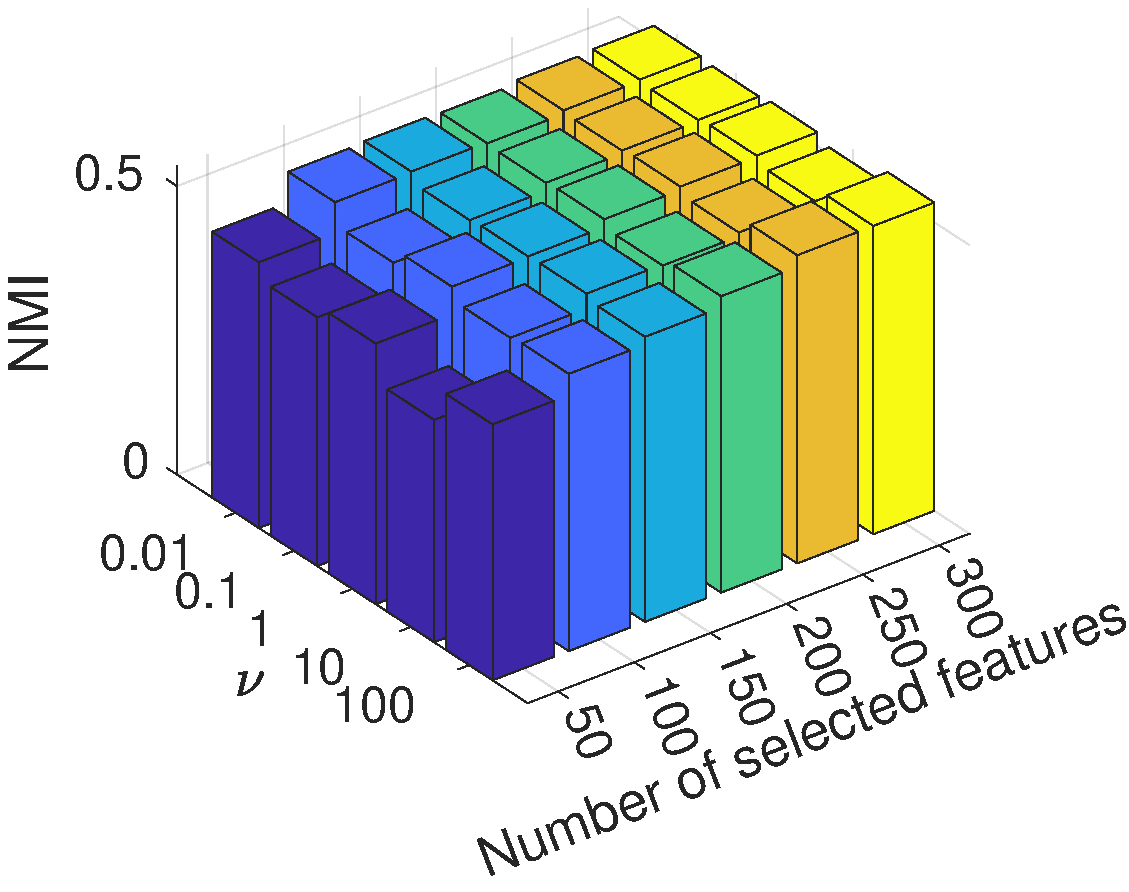
\includegraphics[width=0.33\linewidth]{figures/CPUFS/sensitivity/fmnist_nu.pdf}}
    \subfloat[FashionMNIST ($\alpha$)\label{fig:f2}]{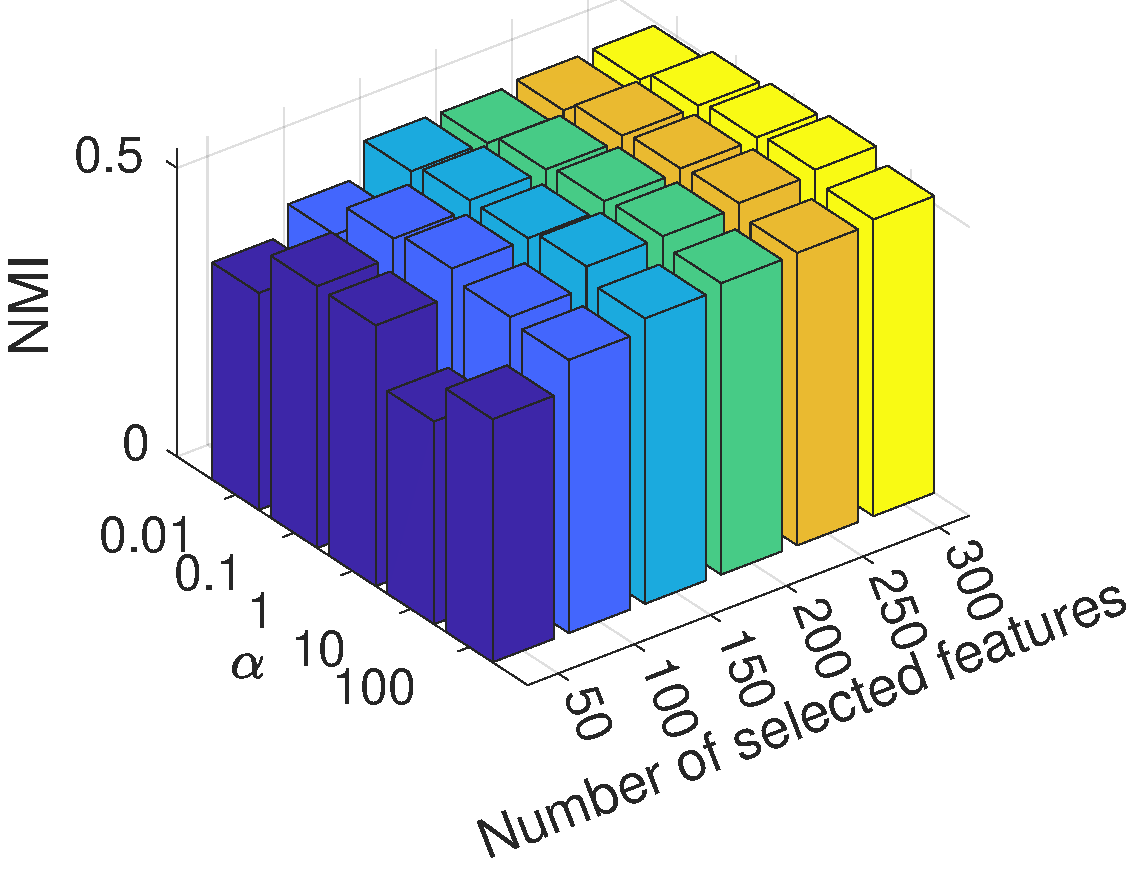
\includegraphics[width=0.33\linewidth]{figures/CPUFS/sensitivity/fmnist_alpha.pdf}}
    \subfloat[FashionMNIST ($\beta$)\label{fig:f3}]{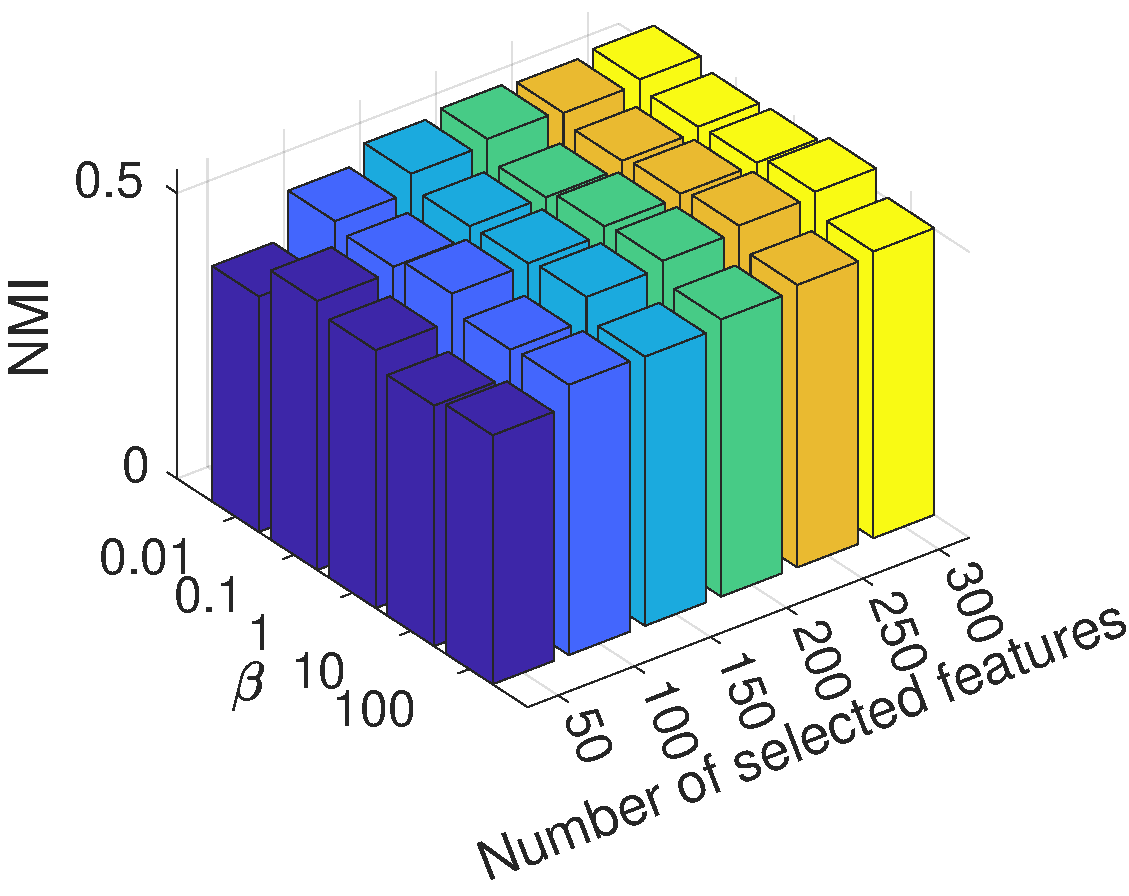
\includegraphics[width=0.33\linewidth]{figures/CPUFS/sensitivity/fmnist_beta.pdf}}\\
    \subfloat[COIL20 ($\nu$)\label{fig:l1}] {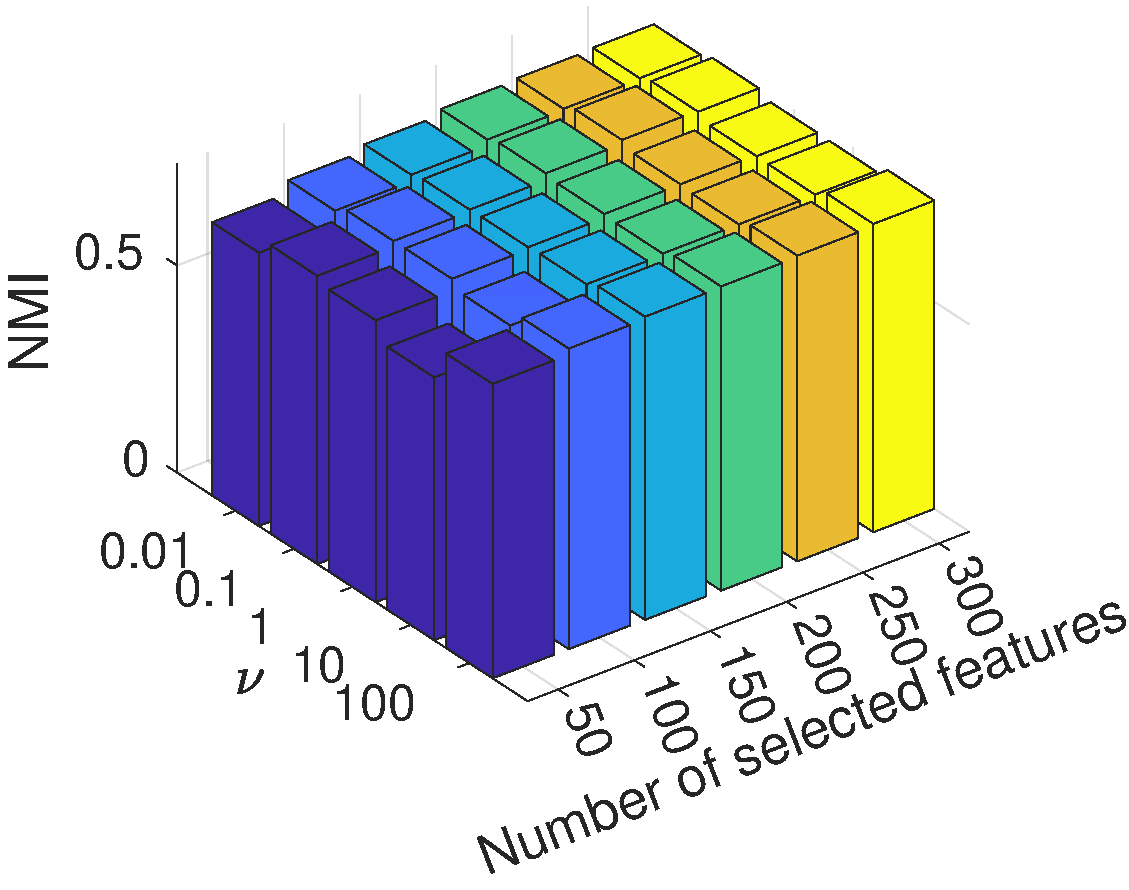
\includegraphics[width=0.33\linewidth]{figures/CPUFS/sensitivity/COIL20_nu.pdf}}
    \subfloat[COIL20 ($\alpha$)\label{fig:l2}]{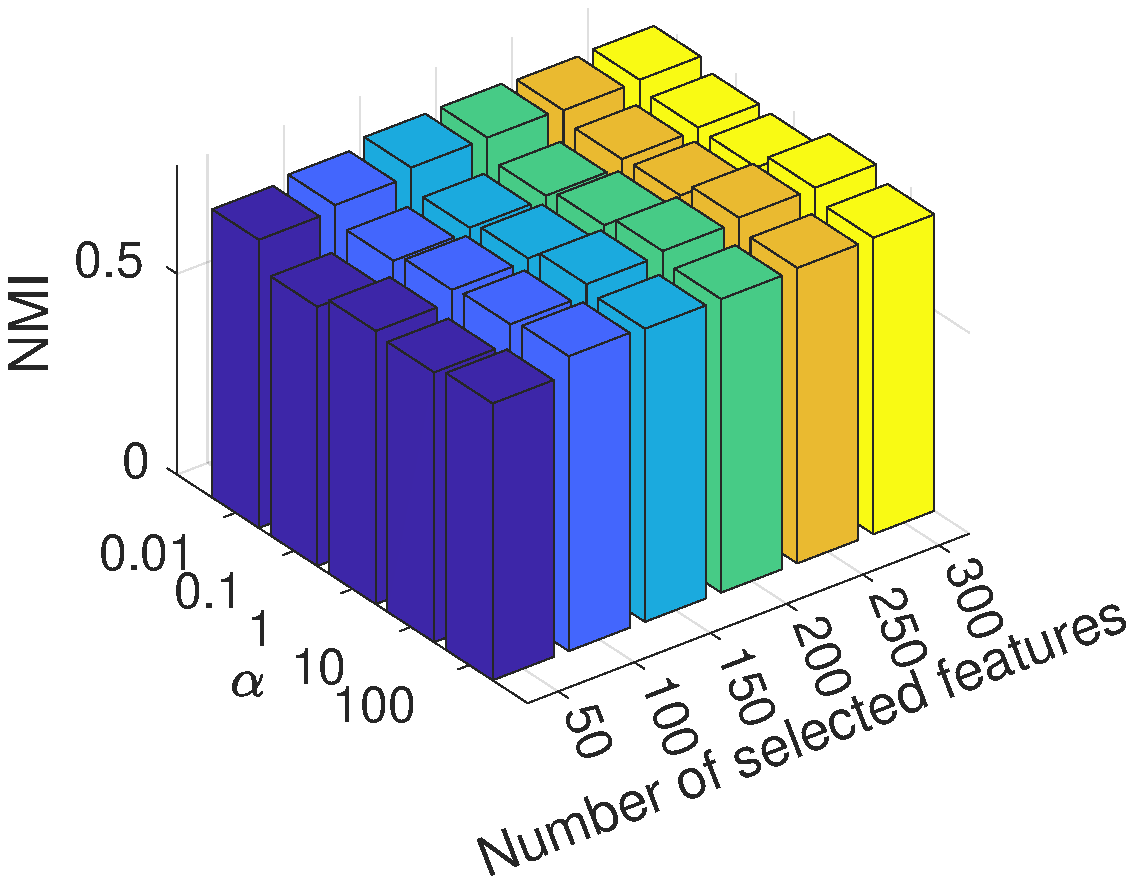
\includegraphics[width=0.33\linewidth]{figures/CPUFS/sensitivity/COIL20_alpha.pdf}}
    \subfloat[COIL20 ($\beta$)\label{fig:l3}]{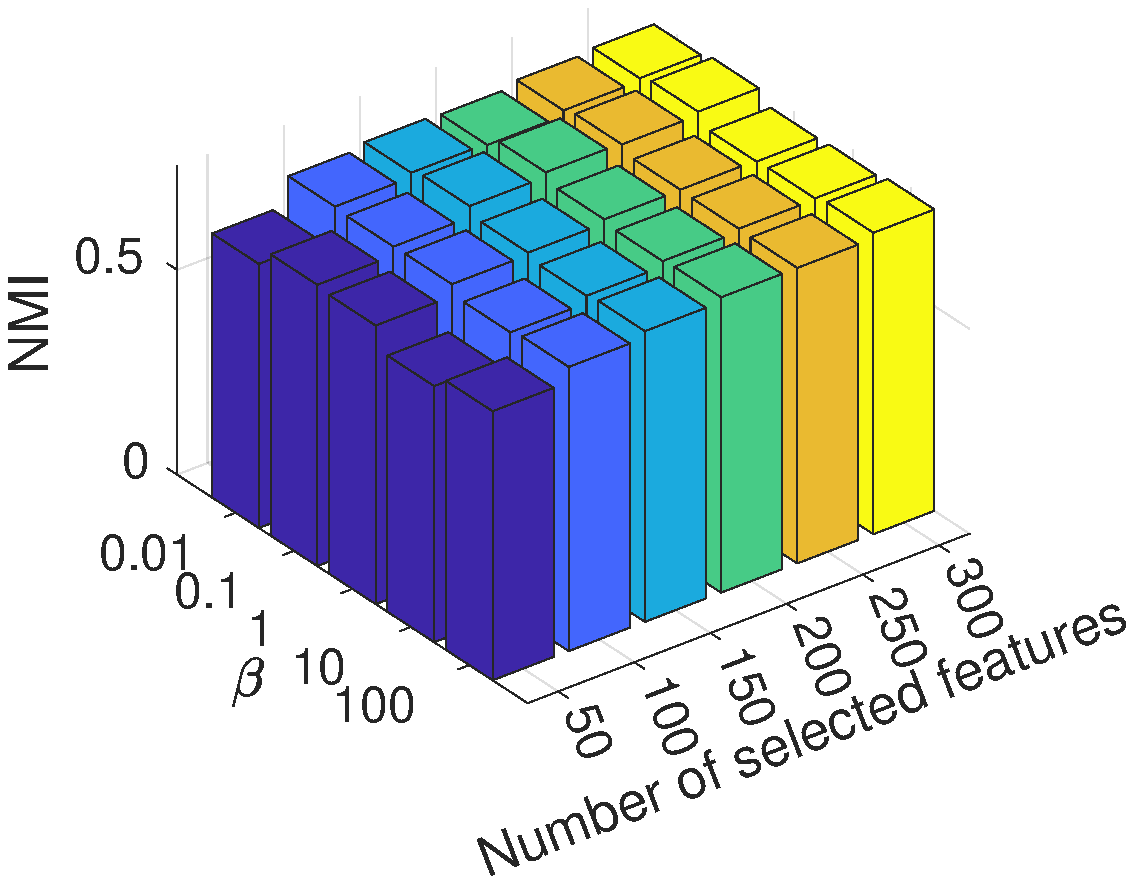
\includegraphics[width=0.33\linewidth]{figures/CPUFS/sensitivity/COIL20_beta.pdf}}\\
    \subfloat[UMIST ($\nu$)\label{fig:w1}] {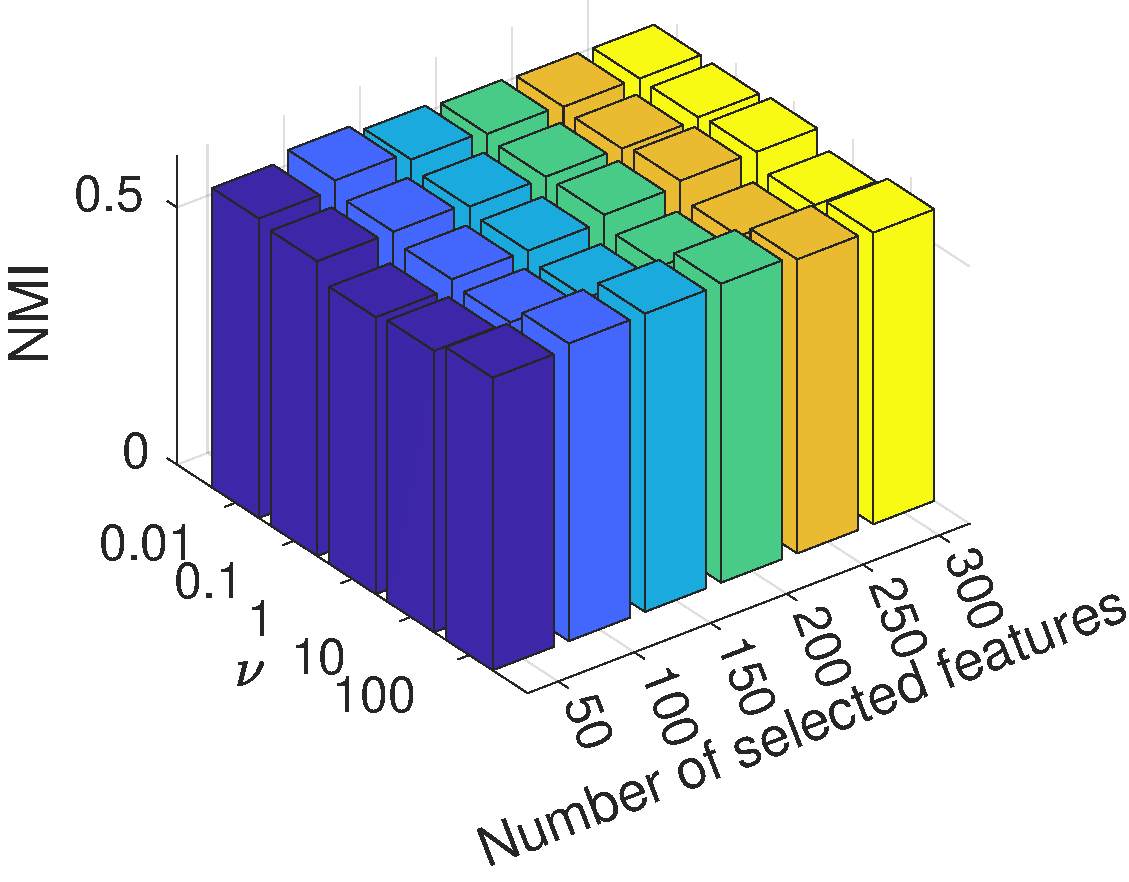
\includegraphics[width=0.33\linewidth]{figures/CPUFS/sensitivity/umist_nu.pdf}}
    \subfloat[UMIST ($\alpha$)\label{fig:w2}]{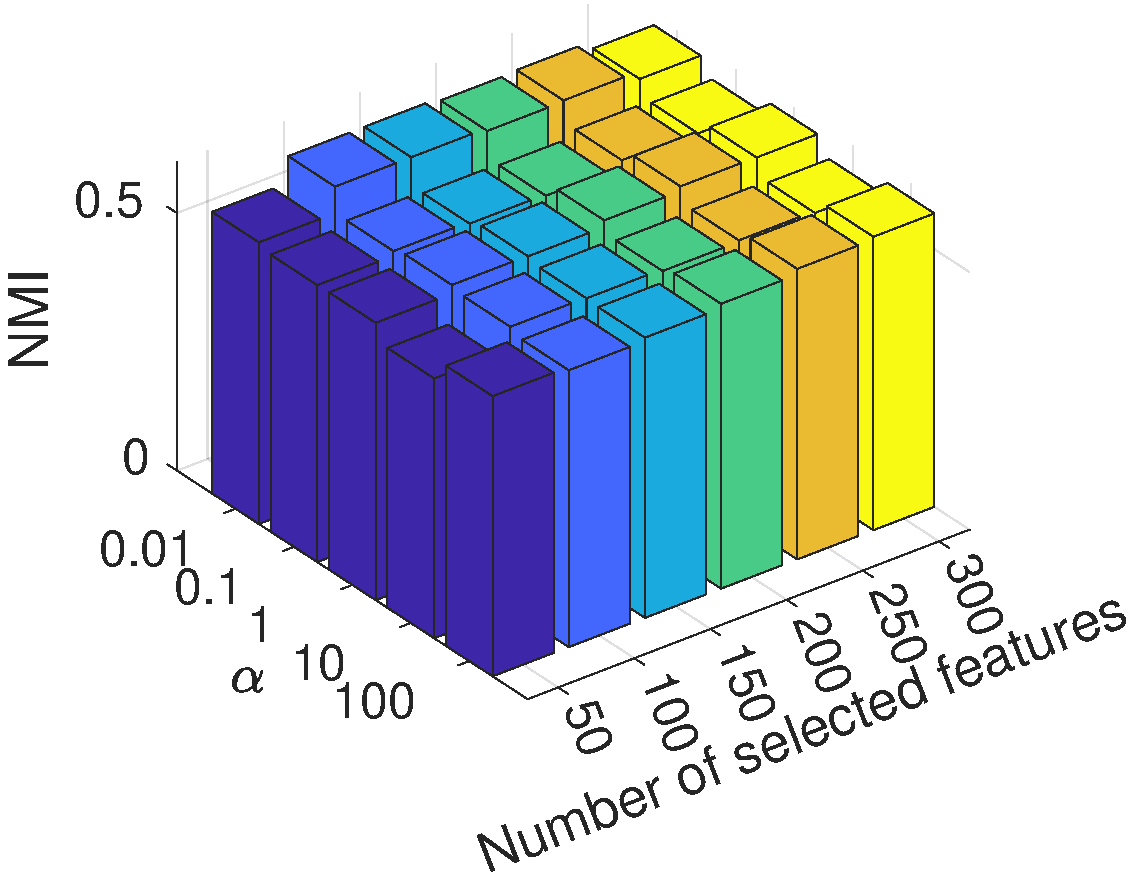
\includegraphics[width=0.33\linewidth]{figures/CPUFS/sensitivity/umist_alpha.pdf}}
    \subfloat[UMIST ($\beta$)\label{fig:w3}]{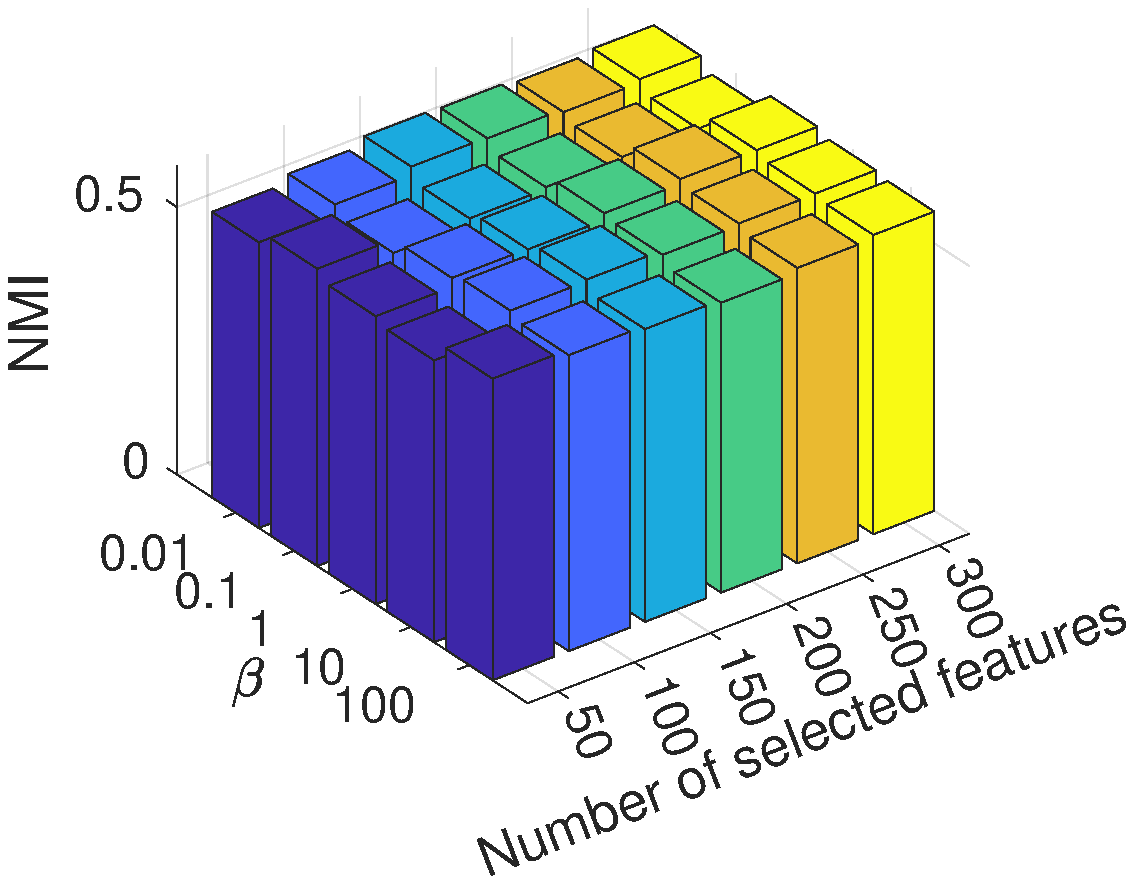
\includegraphics[width=0.33\linewidth]{figures/CPUFS/sensitivity/umist_beta.pdf}}
    \caption{CPUFS方法在FashionMNIST、COIL20与UMIST数据集上的参数敏感度分析}
    \label{fig:sensitivity}
\end{figure}
    
\subsection{参数敏感度分析}
\esubsection{Parameter Sensitivity Analysis}
本节分析CPUFS方法中的参数$\nu$、$\alpha$以及$\beta$对其特征选择性能的影响。具体来说,这些参数交替地在范围$\{10^{-2},10^{-1},1,10,10^{2}\}$内被调整,并且当某个参数被调整时,其余参数均被固定为$1$,然后记录在所有可能的参数组合下CPUFS方法的特征选择性能(由NMI来评价)。实验结果如\reffig{fig:sensitivity}所示。由\reffig{fig:sensitivity},可以得出以下结论:
\begin{enumerate}
\item 在FashionMNIST和COIL20数据集上,当被选择特征的数量较低时(如$50$或$100$),CPUFS方法的性能对这些参数相对敏感,而在其它情况下对这些参数并不敏感。此外,CPUFS方法的性能与被选择特征的数量大致呈正相关关系。
\item 在UMIST数据集上,CPUFS方法的性能对$\alpha$较为敏感,而对其它参数均不敏感。此外,CPUFS方法的性能与被选择特征的数量也不存在显著的相关性。
\end{enumerate}
% 总体而言,CPUFS方法的性能相对于这些参数是较为稳定的。

\subsection{优化效率与收敛性分析}
\esubsection{Optimization Efficiency and Convergence Analyses}
本节首先分析CPUFS方法的优化效率。本文曾在\refsection{sec:companal}分析道,CPUFS方法的优化算法的计算复杂度与数据中的特征数量仅呈线性关系。为了进一步说明理论分析,分别在Pixraw10P、Orlraws10P以及JAFFE数据集上(这三个数据集具有最大的特征数量,因此它们更适合于比较优化效率)运行CPUFS、NDFS、UDFS与RSFS方法(所有方法的所有参数均被固定为$1$),然后记录这四个方法在这三个数据集上的$50$次迭代内的累积时间消耗。实验结果如\reffig{fig:runtime}所示。可以观察到,CPUFS方法与NDFS、UDFS和RSFS方法相比具有明显的优化效率优势,而这个现象符合本文的计算复杂度理论。

\begin{figure}[!t]
    \centering
    \subfloat[Pixraw10P\label{fig:r1}]{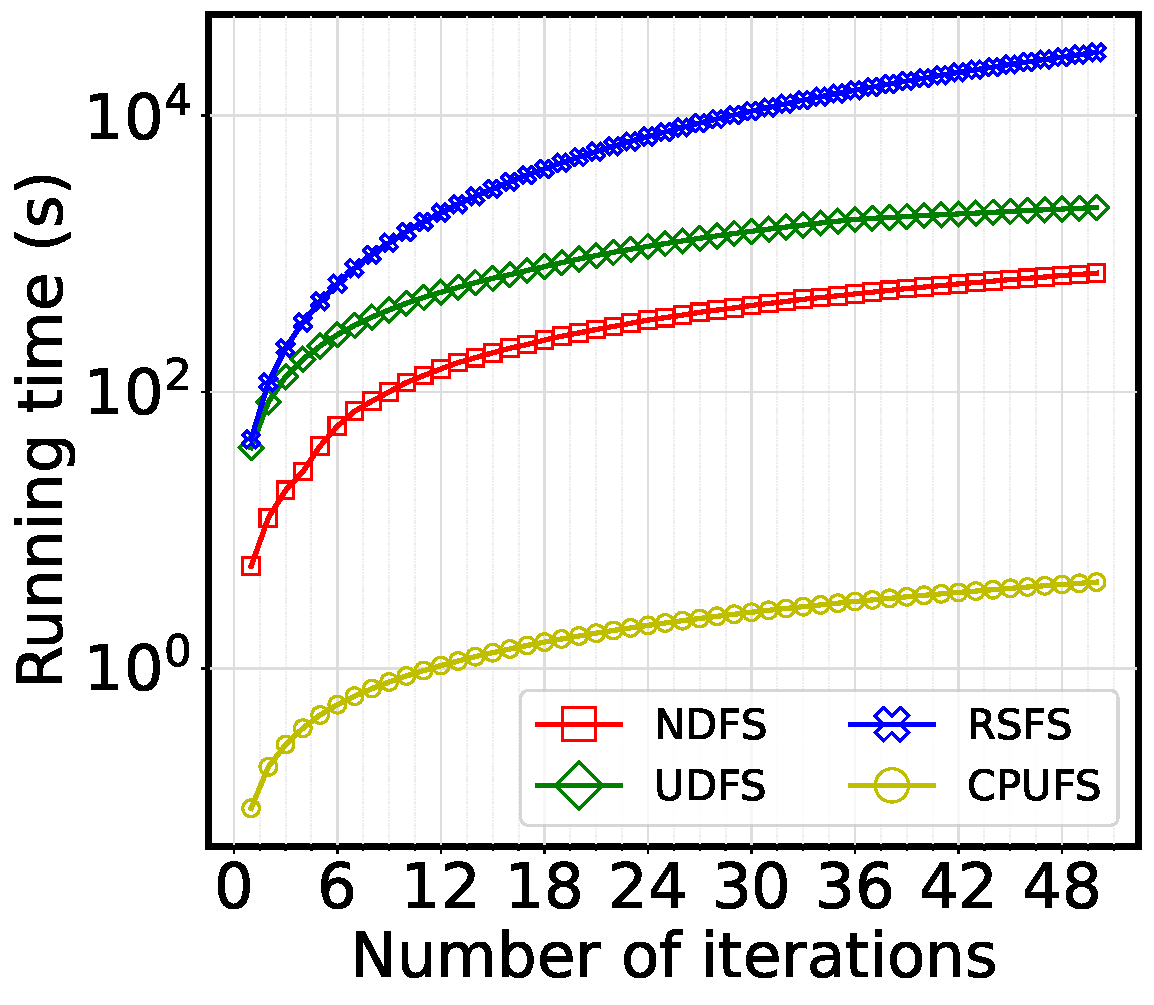
\includegraphics[width=0.33\linewidth]{figures/CPUFS/runtime/CPUFStime_Pixraw10P.pdf}}
    \subfloat[Orlraws10P\label{fig:r2}]{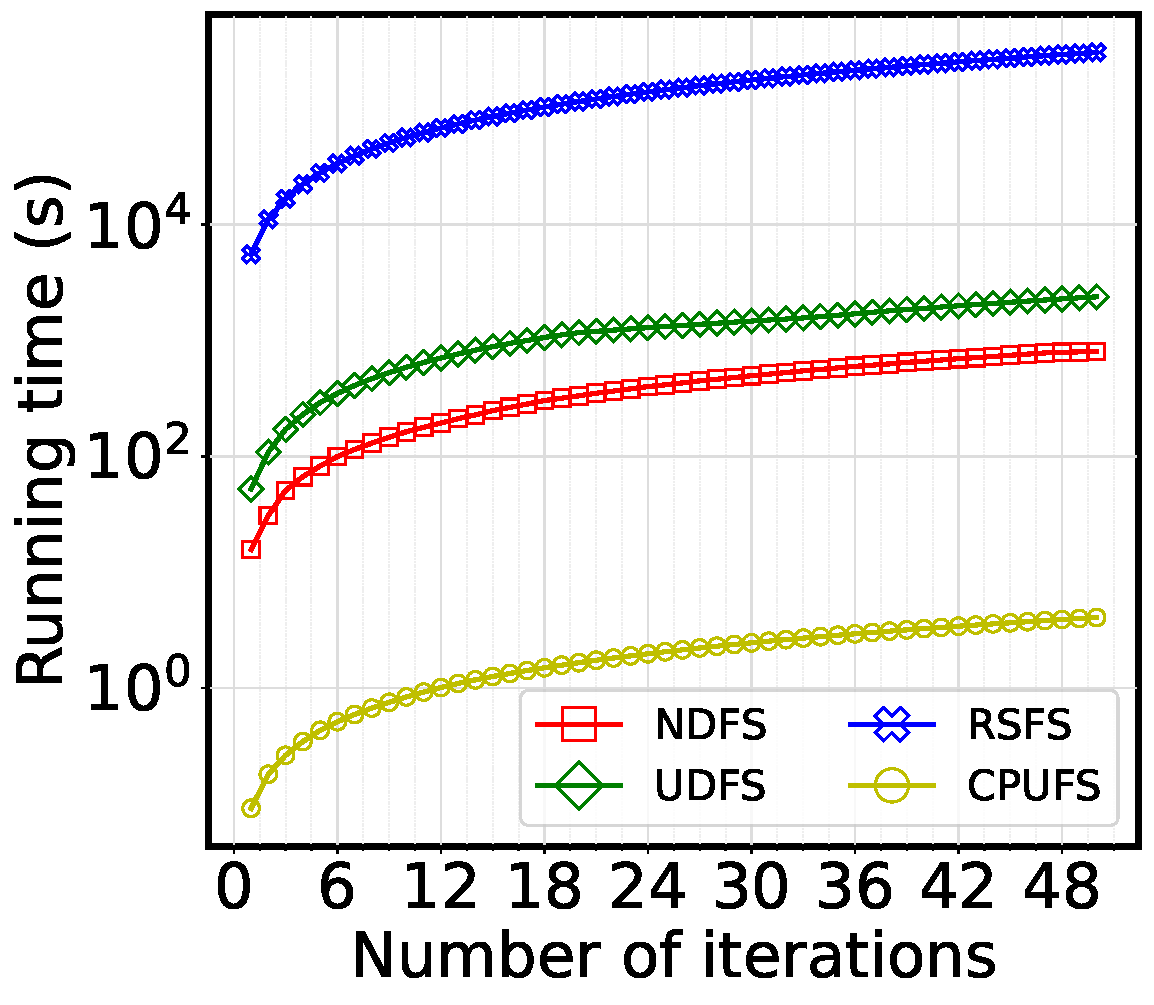
\includegraphics[width=0.33\linewidth]{figures/CPUFS/runtime/CPUFStime_Orlraws10P.pdf}}
    \subfloat[JAFFE\label{fig:r3}]{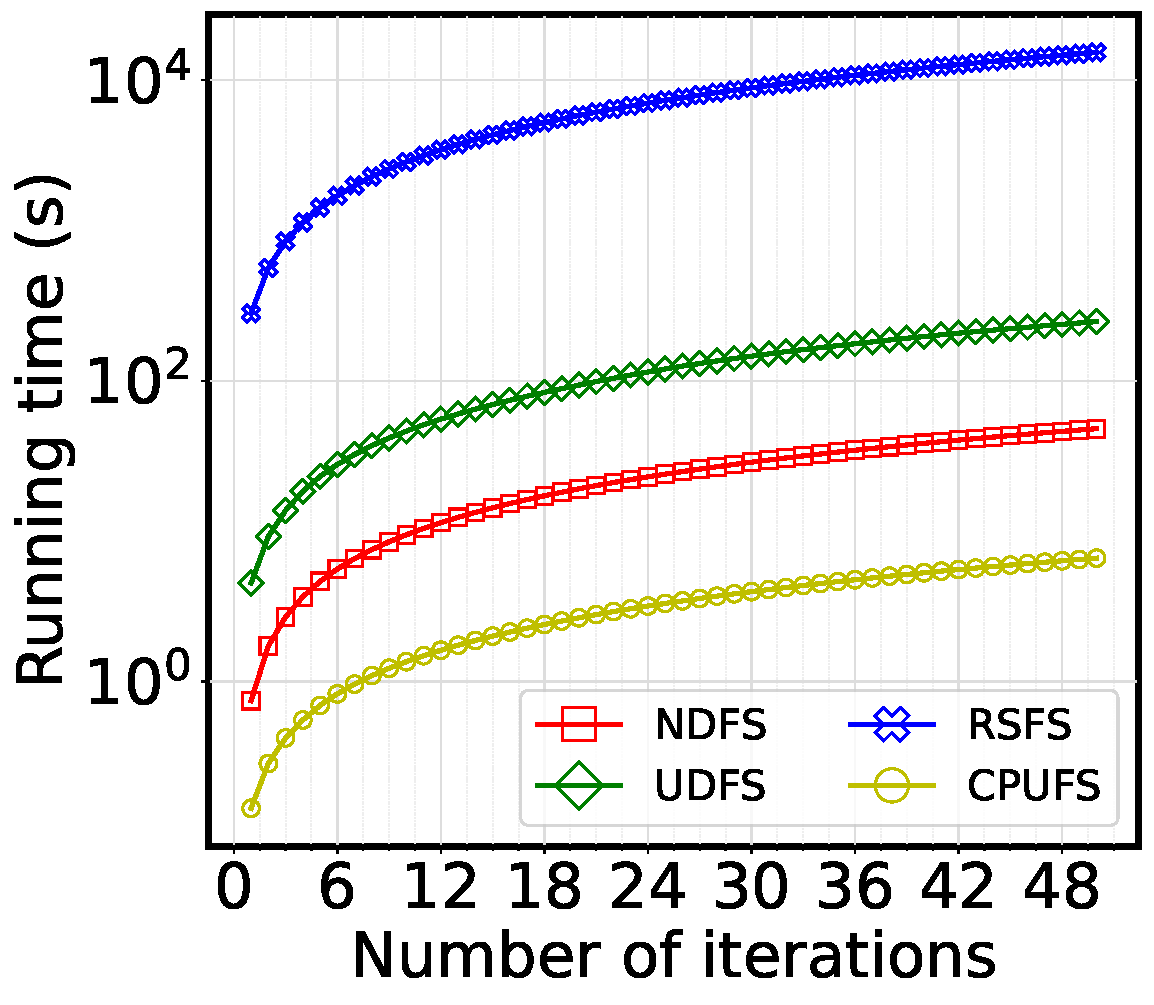
\includegraphics[width=0.33\linewidth]{figures/CPUFS/runtime/CPUFStime_Jaffe.pdf}}
    \caption{CPUFS在Pixraw10P、Orlraws10P与JAFFE数据集上的优化效率分析}
    \label{fig:runtime}
\end{figure}
    
\begin{figure}[!t]
    \centering
    \subfloat[FashionMNIST\label{fig:c1}]{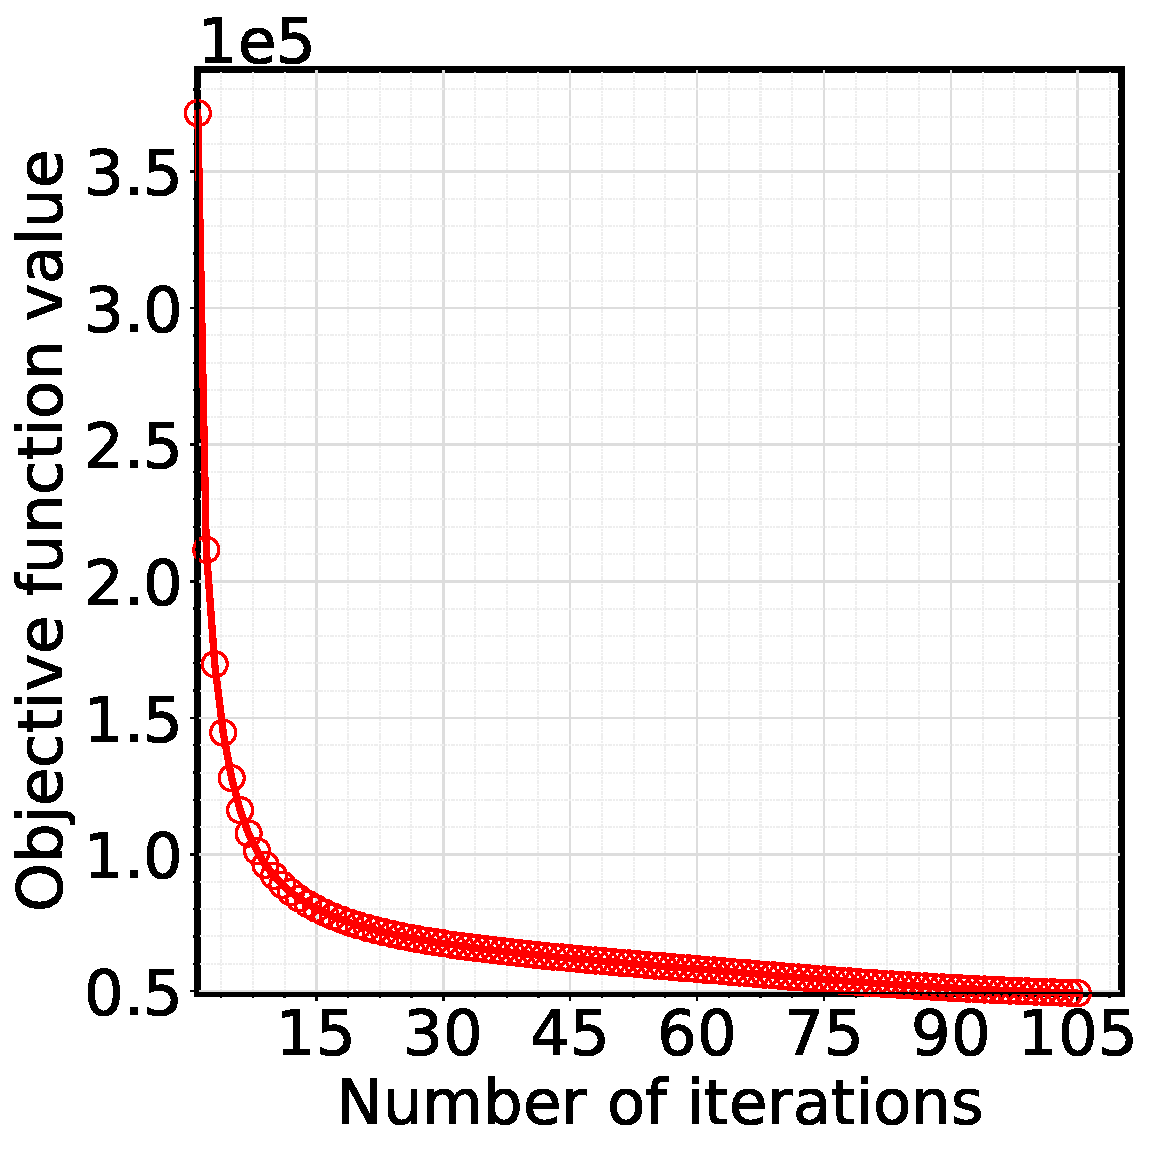
\includegraphics[width=0.33\linewidth]{figures/CPUFS/convergence/loss_fmnist.pdf}}
    \subfloat[COIL20\label{fig:c2}]{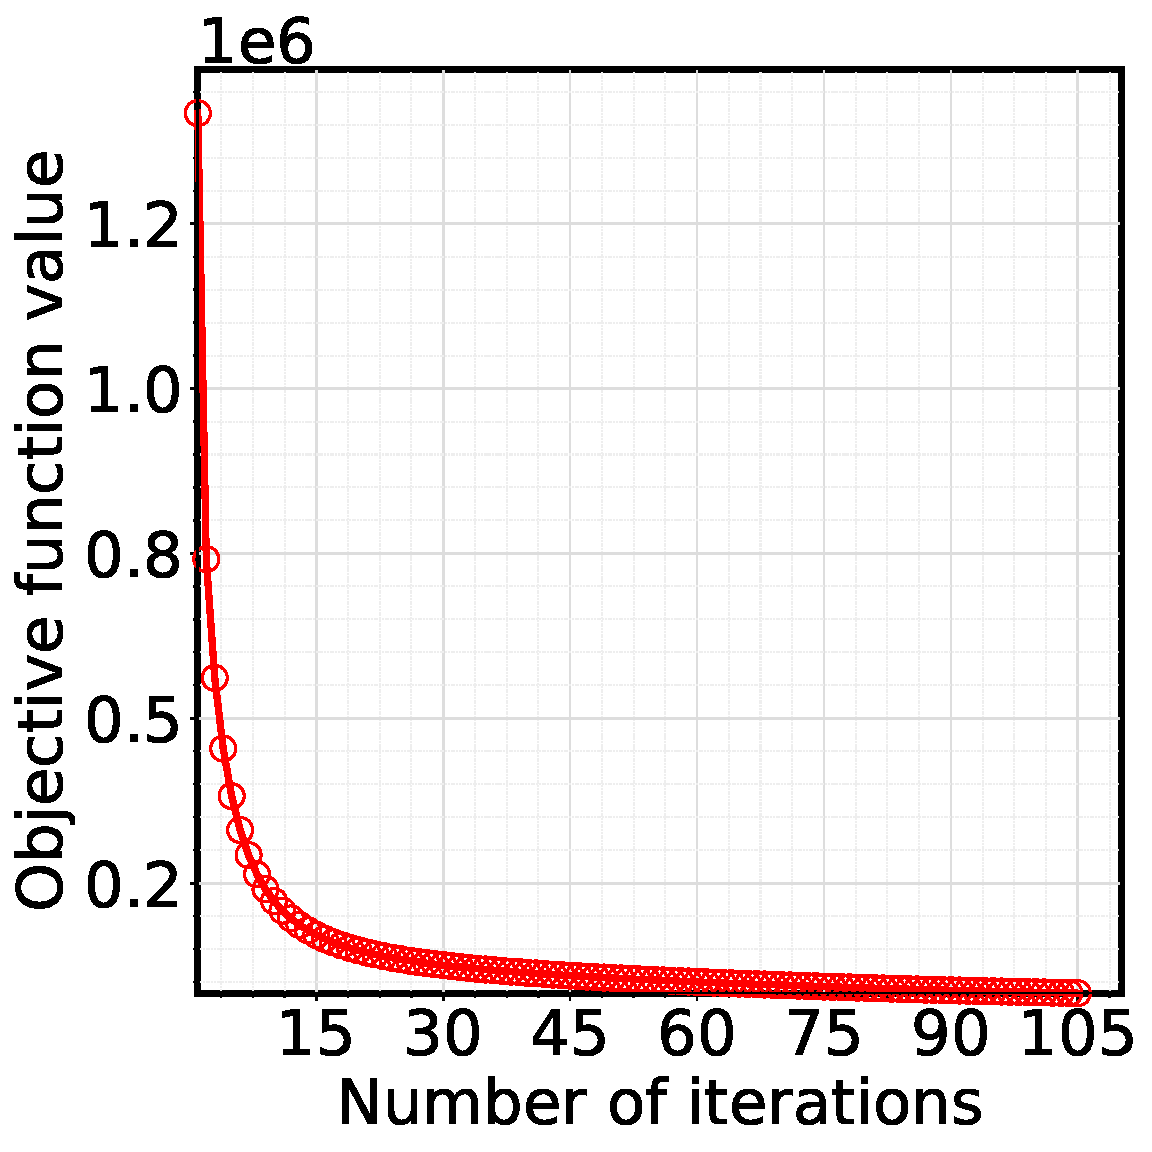
\includegraphics[width=0.33\linewidth]{figures/CPUFS/convergence/loss_COIL20.pdf}}
    \subfloat[UMIST\label{fig:c3}]{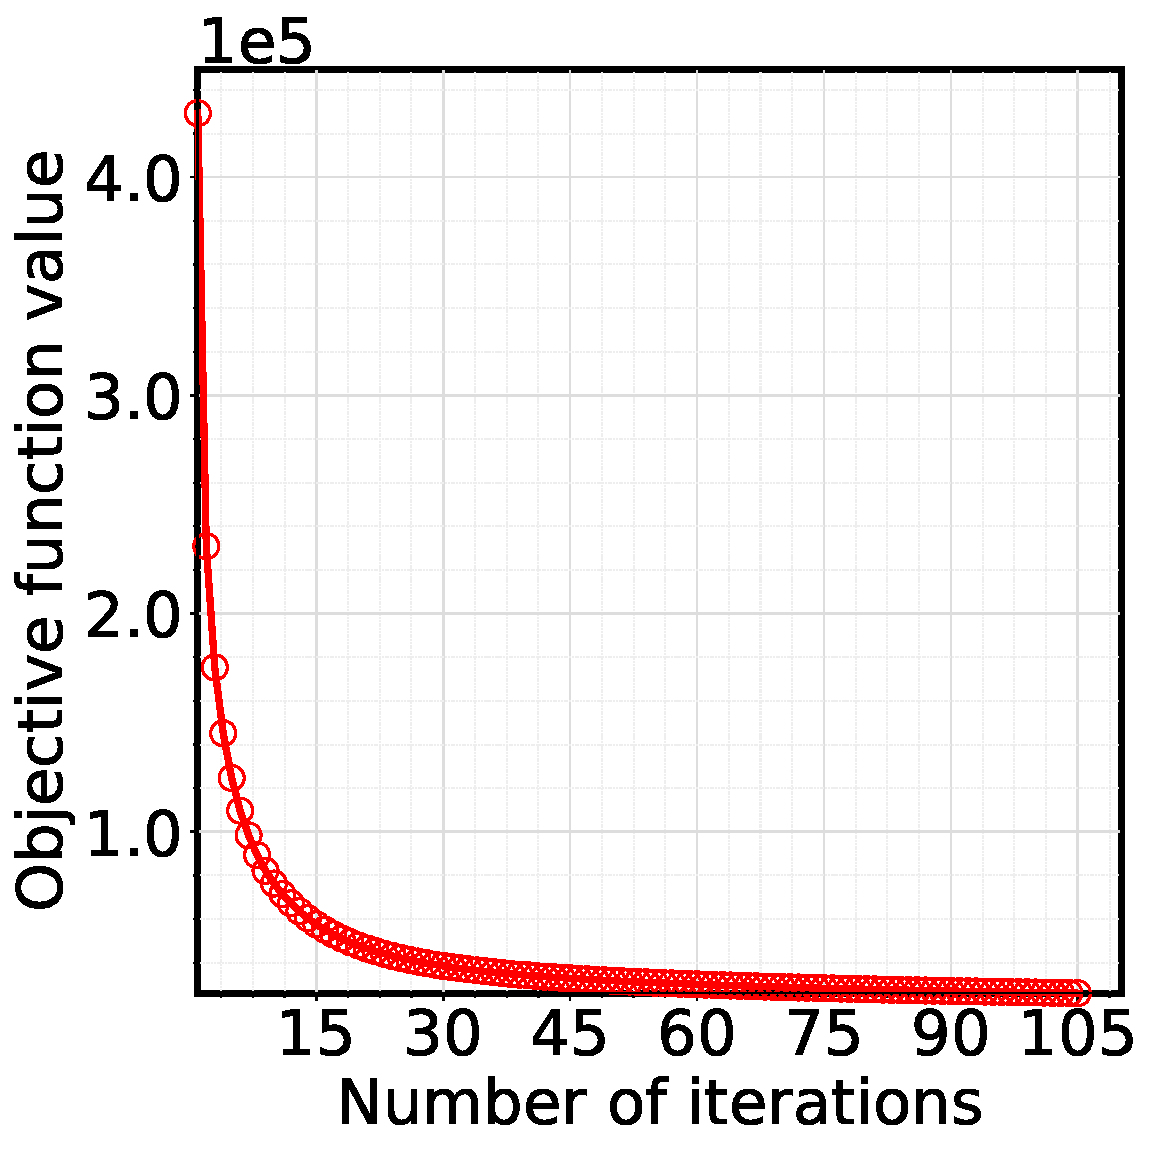
\includegraphics[width=0.33\linewidth]{figures/CPUFS/convergence/loss_umist.pdf}}
    \caption{CPUFS方法在FashionMNIST、COIL20以及UMIST数据集上的收敛性分析}
    \label{fig:converge}
\end{figure}

% \subsection{实验四:收敛性分析}
% \esubsection{Experiment 4: Convergence Analysis}
本节接下来分析CPUFS方法的优化算法的收敛速度。具体来讲,在FashionMNIST、COIL20以及UMIST数据集上运行CPUFS方法(其所有参数均被固定为$1$),并记录其目标函数在每次迭代内的具体数值。记录的目标函数值曲线如\reffig{fig:converge}所示。从\reffig{fig:converge}中可以发现,在这三个数据集上,CPUFS的目标函数值均是单调下降的,而这符合本文的收敛性理论。此外,还可以发现,CPUFS的目标函数值在仅数十次迭代后便降至较低水平,而这反映了CPUFS方法的优化算法的高效性。

\begin{table}[!ht]
    \caption{CPUFS方法与RUFS方法在八个数据集上所选择特征的可视化}\label{tab:visulization}
    \begin{tabular}{>{\centering\arraybackslash}p{0.95in}>{\centering\arraybackslash}p{1.0in}>{\centering\arraybackslash}p{1.0in}>{\centering\arraybackslash}p{1.0in}>{\centering\arraybackslash}p{1.0in}}
        \toprule \diagbox[width=1.2in]{方法}{数据集} & ORL & JAFFE & OCTMNIST & FashionMNIST \\
        \midrule 原始图像 & \parbox[c]{1.0in}{
        
\includegraphics[width=1\linewidth]{figures/CPUFS/visualization/feaOriginal_ORL.pdf}} & \parbox[c]{1.0in}{
        
\includegraphics[width=1\linewidth]{figures/CPUFS/visualization/feaOriginal_JAFFE.pdf}} & \parbox[c]{1.0in}{
        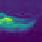
\includegraphics[width=1\linewidth]{figures/CPUFS/visualization/feaOriginal_octmnist.pdf}} & \parbox[c]{1.0in}{
        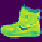
\includegraphics[width=1\linewidth]{figures/CPUFS/visualization/feaOriginal_fmnist.pdf}} \\\addlinespace[0.5em]
        CPUFS & \parbox[c]{1.0in}{
        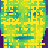
\includegraphics[width=1\linewidth]{figures/CPUFS/visualization/feaCPUFS_ORL.pdf}} & \parbox[c]{1.0in}{
        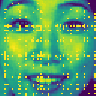
\includegraphics[width=1\linewidth]{figures/CPUFS/visualization/feaCPUFS_JAFFE.pdf}} & \parbox[c]{1.0in}{
        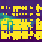
\includegraphics[width=1\linewidth]{figures/CPUFS/visualization/feaCPUFS_octmnist.pdf}} & \parbox[c]{1.0in}{
        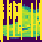
\includegraphics[width=1\linewidth]{figures/CPUFS/visualization/feaCPUFS_fmnist.pdf}} \\\addlinespace[0.5em]
        RUFS & \parbox[c]{1.0in}{
        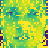
\includegraphics[width=1\linewidth]{figures/CPUFS/visualization/feaRUFS_ORL.pdf}} & \parbox[c]{1.0in}{
        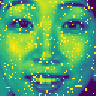
\includegraphics[width=1\linewidth]{figures/CPUFS/visualization/feaRUFS_JAFFE.pdf}} & \parbox[c]{1.0in}{
        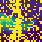
\includegraphics[width=1\linewidth]{figures/CPUFS/visualization/feaRUFS_octmnist.pdf}} & \parbox[c]{1.0in}{
        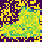
\includegraphics[width=1\linewidth]{figures/CPUFS/visualization/feaRUFS_fmnist.pdf}} \\
        \midrule\midrule \diagbox[width=1.2in]{方法}{数据集} & COIL20 & BreastMNIST & Pixraw10P & Orlraws10P \\
        \midrule 原始图像 & \parbox[c]{1.0in}{
        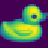
\includegraphics[width=1\linewidth]{figures/CPUFS/visualization/feaOriginal_COIL20.pdf}} & \parbox[c]{1.0in}{
        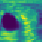
\includegraphics[width=1\linewidth]{figures/CPUFS/visualization/feaOriginal_breastmnist.pdf}} & \parbox[c]{1.0in}{
        
\includegraphics[width=1\linewidth]{figures/CPUFS/visualization/feaOriginal_pixraw10P.pdf}} & \parbox[c]{1.0in}{
        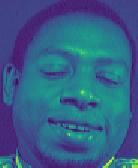
\includegraphics[width=1\linewidth]{figures/CPUFS/visualization/feaOriginal_orlraws10P.pdf}} \\\addlinespace[0.5em]
        CPUFS & \parbox[c]{1.0in}{
        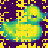
\includegraphics[width=1\linewidth]{figures/CPUFS/visualization/feaCPUFS_COIL20.pdf}} & \parbox[c]{1.0in}{
        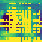
\includegraphics[width=1\linewidth]{figures/CPUFS/visualization/feaCPUFS_breastmnist.pdf}} & \parbox[c]{1.0in}{
        
\includegraphics[width=1\linewidth]{figures/CPUFS/visualization/feaCPUFS_pixraw10P.pdf}} & \parbox[c]{1.0in}{
        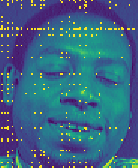
\includegraphics[width=1\linewidth]{figures/CPUFS/visualization/feaCPUFS_orlraws10P.pdf}} \\\addlinespace[0.5em]
        RUFS & \parbox[c]{1.0in}{
        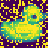
\includegraphics[width=1\linewidth]{figures/CPUFS/visualization/feaRUFS_COIL20.pdf}} & \parbox[c]{1.0in}{
        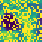
\includegraphics[width=1\linewidth]{figures/CPUFS/visualization/feaRUFS_breastmnist.pdf}} & \parbox[c]{1.0in}{
        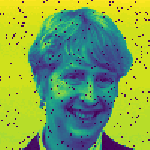
\includegraphics[width=1\linewidth]{figures/CPUFS/visualization/feaRUFS_pixraw10P.pdf}} & \parbox[c]{1.0in}{
        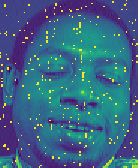
\includegraphics[width=1\linewidth]{figures/CPUFS/visualization/feaRUFS_orlraws10P.pdf}} \\
        \bottomrule
    \end{tabular}
  \end{table}

\subsection{被选择特征的可视化分析}\label{sec:visualization}
\esubsection{Visual Analysis of the Selected Features}
本文曾在\refsection{sec:design-fsmatrix}理论地分析道,在CPUFS方法中,来自数据同一行或同一列的特征具有相互关联的重要性权重。现在展示这种相关性在现实情况下的表征。具体来讲,对于某一数据集,首先检索$300$个就NMI而言表现最好的特征(即该$300$个特征就是达到\reffig{fig:clusnmi}中性能的那些特征)。之后,从该数据集中随机采样一张图像,然后在这张图像上掩盖这$300$个特征并展示。此外,由于CPUFS方法与RUFS方法较为相似,因此本文还使用了同样的方法可视化了RUFS方法所选择的特征。在ORL、JAFFE、OCTMNIST、FashionMNIST、COIL20、BreastMNIST、Pixraw10P以及Orlraws10P这八个数据集上进行了上述实验,实验结果如\reftab{tab:visulization}所示。从\reftab{tab:visulization}可以看出,由CPUFS方法所选择的特征在空间上具有较强的相关性:
\begin{enumerate}
    \item 在FashionMNIST、COIL20以及Pixraw10P数据集上,被选择的特征在垂直方向上具有清晰的结构特性;
    \item 在ORL数据集上,被选择的特征更倾向于聚集在较小的矩形子区域内;
    \item 在JAFFE和Orlraws10P数据集上,被选择的特征显示出了明显的网格状结构;
    \item 在OCTMNIST和BreastMNIST数据集上,被选择的特征更倾向于聚集在一起。
\end{enumerate}
然而,由RUFS方法所选择的特征并没有显示出这样的效果。这种现象充分展示了CPUFS方法作为面向张量的无监督特征选择方法的有效性。本文认为,CPUFS方法的性能提升主要归因于其所选特征的更好结构。

% \begin{figure}[!t]
%     \centering
%     \subfloat[FashionMNIST] {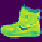
\includegraphics[width=0.32\linewidth]{figures/CPUFS/visualization/feaOriginal_fmnist.pdf}}
%     \hspace{0.01\linewidth}
%     \subfloat[FashionMNIST (CPUFS)]{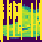
\includegraphics[width=0.32\linewidth]{figures/CPUFS/visualization/feaCPUFS_fmnist.pdf}}
%     \hspace{0.01\linewidth}
%     \subfloat[FashionMNIST (RUFS)] {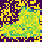
\includegraphics[width=0.32\linewidth]{figures/CPUFS/visualization/feaRUFS_fmnist.pdf}}\\
%     \subfloat[COIL20] {\includegraphics[width=0.32\linewidth]{figures/CPUFS/visualization/feaOriginal_COIL20.pdf}}
%     \hspace{0.01\linewidth}
%     \subfloat[COIL20 (CPUFS)]{\includegraphics[width=0.32\linewidth]{figures/CPUFS/visualization/feaCPUFS_COIL20.pdf}}
%     \hspace{0.01\linewidth}
%     \subfloat[COIL20 (RUFS)] {\includegraphics[width=0.32\linewidth]{figures/CPUFS/visualization/feaRUFS_COIL20.pdf}}\\
%     \subfloat[ORL] {\includegraphics[width=0.32\linewidth]{figures/CPUFS/visualization/feaOriginal_ORL.pdf}}
%     \hspace{0.01\linewidth}
%     \subfloat[ORL (CPUFS)]{\includegraphics[width=0.32\linewidth]{figures/CPUFS/visualization/feaCPUFS_ORL.pdf}}
%     \hspace{0.01\linewidth}
%     \subfloat[ORL (RUFS)] {\includegraphics[width=0.32\linewidth]{figures/CPUFS/visualization/feaRUFS_ORL.pdf}}\\
%     \subfloat[Pixraw10P] {\includegraphics[width=0.32\linewidth]{figures/CPUFS/visualization/feaOriginal_pixraw10P.pdf}}
%     \hspace{0.01\linewidth}
%     \subfloat[Pixraw10P (CPUFS)]{\includegraphics[width=0.32\linewidth]{figures/CPUFS/visualization/feaCPUFS_pixraw10P.pdf}}
%     \hspace{0.01\linewidth}
%     \subfloat[Pixraw10P (RUFS)] {\includegraphics[width=0.32\linewidth]{figures/CPUFS/visualization/feaRUFS_pixraw10P.pdf}}\\    
% \end{figure}
% \begin{figure}[!t]
%     \ContinuedFloat
%     \centering
%     \subfloat[Orlraws10P] {\includegraphics[width=0.32\linewidth]{figures/CPUFS/visualization/feaOriginal_orlraws10P.pdf}}
%     \hspace{0.01\linewidth}
%     \subfloat[Orlraws10P (CPUFS)]{\includegraphics[width=0.32\linewidth]{figures/CPUFS/visualization/feaCPUFS_orlraws10P.pdf}}
%     \hspace{0.01\linewidth}
%     \subfloat[Orlraws10P (RUFS)] {\includegraphics[width=0.32\linewidth]{figures/CPUFS/visualization/feaRUFS_orlraws10P.pdf}}\\
%     \subfloat[JAFFE] {\includegraphics[width=0.32\linewidth]{figures/CPUFS/visualization/feaOriginal_jaffe.pdf}}
%     \hspace{0.01\linewidth}
%     \subfloat[JAFFE (CPUFS)]{\includegraphics[width=0.32\linewidth]{figures/CPUFS/visualization/feaCPUFS_JAFFE.pdf}}
%     \hspace{0.01\linewidth}
%     \subfloat[JAFFE (RUFS)] {\includegraphics[width=0.32\linewidth]{figures/CPUFS/visualization/feaRUFS_JAFFE.pdf}}\\
%     \subfloat[BreastMNIST] {\includegraphics[width=0.32\linewidth]{figures/CPUFS/visualization/feaOriginal_breastmnist.pdf}}
%     \hspace{0.01\linewidth}
%     \subfloat[BreastMNIST (CPUFS)]{\includegraphics[width=0.32\linewidth]{figures/CPUFS/visualization/feaCPUFS_breastmnist.pdf}}
%     \hspace{0.01\linewidth}
%     \subfloat[BreastMNIST (RUFS)] {\includegraphics[width=0.32\linewidth]{figures/CPUFS/visualization/feaRUFS_breastmnist.pdf}}\\
%     \subfloat[OCTMNIST] {\includegraphics[width=0.32\linewidth]{figures/CPUFS/visualization/feaOriginal_octmnist.pdf}}
%     \hspace{0.01\linewidth}
%     \subfloat[OCTMNIST (CPUFS)]{\includegraphics[width=0.32\linewidth]{figures/CPUFS/visualization/feaCPUFS_octmnist.pdf}}
%     \hspace{0.01\linewidth}
%     \subfloat[OCTMNIST (RUFS)] {\includegraphics[width=0.32\linewidth]{figures/CPUFS/visualization/feaRUFS_octmnist.pdf}}\\
%     \caption{CPUFS与RUFS在八个数据集上所选择特征的可视化}
%     \label{fig:visulization}
% \end{figure}
% \clearpage
\section{无监督特征提取实验}
\esection{Experiments on Unsupervised Feature Extraction}
% \subsection{实验一:$\ell_{1}$与$\ell_{\infty}$方法和\texorpdfstring{$\ell_{2}$}{L2}方法的性能对比}
% \esubsection{Experiment 1: Comparisons of the $\ell_{1}$ and $\ell_{\infty}$ Methods against the \texorpdfstring{$\ell_{2}$}{L2} Method}
本节将展示无监督特征提取任务的实验结果,并加以分析。
\subsection{性能对比}
\esubsection{Performance Comparison}

\begin{table}[!t]
        \caption{\mbox{$\ell_{1}$、$\ell_{2}$以及$\ell_{\infty}$方法在COIL20数据集上的性能对比}}
        \label{tab:coil}
        \centering
            \begin{tabular}{lcccccc}
    \hline
    \multirow{2}{*}{噪声类型} & \multicolumn{3}{c}{$k$-NN ACC}                                                                         & \multicolumn{3}{c}{SVM ACC}                                                                            \\ \cline{2-7}
                           & $\ell_2$                         & $\ell_1$                         & $\ell_\infty$                    & $\ell_2$                         & $\ell_1$                         & $\ell_\infty$                    \\ \hline
    原始数据               & \textbf{0.9208} & 0.8906                           & {0.8891}       & \textbf{0.9406} & 0.9065                           & 0.9198                           \\
    % \hline\hline
    ms-5-10-20                  & 0.8560                           & 0.8560                           & \textbf{0.8810} & 0.9234                           & 0.9242                           & \textbf{0.9388} \\
    ms-10-10-10 & 0.8435 & 0.8240 & \textbf{0.8990} & 0.9234 & 0.8758 & \textbf{0.9500} \\
    ms-10-20-30 & 0.8224 & 0.7852 & \textbf{0.8406} & 0.9036 & 0.9133 & \textbf{0.9466} \\
    ms-10-30-50 & 0.8221 & 0.8013 & \textbf{0.8721} & 0.9031 & 0.9107 & \textbf{0.9339} \\
    ms-10-50-90 & 0.8128 & 0.7888 & \textbf{0.8664} & 0.9133 & 0.9008 & \textbf{0.9401} \\
    ms-20-20-20 & 0.8159 & 0.8073 & \textbf{0.8698} & 0.9112 & 0.9010 & \textbf{0.9378} \\
    ms-30-30-30 & 0.7901 & 0.8180 & \textbf{0.8768} & 0.9174 & 0.9104 & \textbf{0.9380} \\
    ms-40-40-40 & 0.8076 & 0.8193 & \textbf{0.8964} & 0.9190 & 0.9128 & \textbf{0.9570} \\
    ms-50-50-50 & 0.8250 & 0.8206 & \textbf{0.8680} & 0.9216 & 0.9216 & \textbf{0.9469} \\
    % ms010                  & 0.8068                           & \textbf{0.8836} & {0.8432}       & 0.7211                           & \textbf{0.9307} & 0.8076                           \\
    % ms020                  & 0.5659                           & \textbf{0.8766} & {0.8536}       & 0.4023                           & 0.6763                           & \textbf{0.7685} \\
    % sp002                  & 0.8453                           & 0.8305                           & \textbf{0.8664}       & \textbf{0.9276} & 0.9021                           & 0.9096                           \\
    % sp005                  & 0.8286                           & 0.8237                           & \textbf{0.8721} & 0.9021                           & 0.8938                           & \textbf{0.9026} \\
    % sp007                  & \textbf{0.8372} & 0.8172                           & {0.8076}       & 0.8661                           & 0.8792                           & \textbf{0.8932} \\
    % ms-0-0-0-90                 & 0.8576                           & 0.8375                           & \textbf{0.8826} & 0.9177                           & 0.8977                           & \textbf{0.9187} \\
    ms-5-10-15-20                 & 0.8285                           & 0.7830                           & \textbf{0.8969} & 0.9041                           & 0.8934                           & \textbf{0.9346} \\
    ms-10-10-10-10 & 0.8320 & 0.8391 & \textbf{0.8482} & \textbf{0.9260} & 0.9156 & 0.9115 \\
    ms-10-20-30-40                 & 0.7526                           & 0.7049                           & \textbf{0.8534} & 0.8945                           & 0.8734                           & \textbf{0.9352} \\
    % ms-10-20-30-90 & \textbf{0.7883} & 0.7513 & 0.7781 & 0.8971 & 0.8956 & \textbf{0.9216} \\
    % ms1239                 & \textbf{0.7883} & 0.7513                           & {0.7781}       & 0.8971                           & 0.8956                           & \textbf{0.9216} \\
    ms-10-30-50-70                 & 0.7940                           & 0.7776                           & \textbf{0.8555} & 0.8729                           & 0.9156                           & \textbf{0.9344} \\
    ms-20-20-20-20 & 0.7716 & \textbf{0.8247} & 0.8063 & 0.9078 & 0.9086 & \textbf{0.9245} \\
    ms-30-30-30-30 & 0.7615 & 0.7880 & \textbf{0.8010} & 0.9125 & 0.9159 & \textbf{0.9430} \\
    ms-40-40-40-40 & 0.7596 & 0.7802 & \textbf{0.8526} & 0.9201 & 0.9281 & \textbf{0.9549} \\
    ms-50-50-50-50 & 0.7721 & 0.7974 & \textbf{0.8104} & 0.9190 & 0.9143 & \textbf{0.9385} \\
    \hline\hline
    % sp-1-2-10                  & 0.8461                           & 0.8471                           & \textbf{0.8922} & 0.9180                           & 0.9005                           & \textbf{0.9292} \\
    sp-5-10-20 & 0.8029 & 0.8109 & \textbf{0.8839} & 0.9115 & 0.9026 & \textbf{0.9383} \\
    sp-10-10-10 & 0.7865 & 0.7492 & \textbf{0.8664} & 0.9065 & 0.8841 & \textbf{0.9320} \\
    sp-10-20-30 & 0.7969 & 0.7414 & \textbf{0.8766} & 0.8922 & 0.7859 & \textbf{0.9336} \\
    sp-10-30-50 & 0.7865 & 0.8318 & \textbf{0.8846} & 0.8992 & 0.8901 & \textbf{0.9164} \\
    sp-10-50-90 & 0.8227 & 0.6411 & \textbf{0.8701} & 0.8938 & 0.7299 & \textbf{0.9107} \\
    sp-20-20-20 & 0.7802 & 0.8255 & \textbf{0.8646} & 0.9057 & 0.8896 & \textbf{0.9313} \\
    sp-30-30-30 & 0.7896 & 0.7422 & \textbf{0.8789} & 0.8932 & 0.8401 & \textbf{0.9089} \\
    sp-40-40-40 & 0.8013 & 0.8253 & \textbf{0.8685} & 0.8948 & 0.8690 & \textbf{0.9242} \\
    sp-50-50-50 & 0.8216 & 0.7901 & \textbf{0.8508} & 0.8776 & \textbf{0.8961} & 0.8779 \\
    % sp-0-0-0-20                 & 0.8362                           & 0.8143                           & \textbf{0.9089} & 0.9172                           & 0.9120                           & \textbf{0.9385} \\
    % sp-1-2-5-10                 & 0.8370                           & 0.8292                           & \textbf{0.8966} & 0.9141                           & 0.9062                           & \textbf{0.9398} \\
    sp-5-10-15-20                 & 0.7701                           & 0.7482                           & \textbf{0.8453} & 0.8849                           & 0.8388                           & \textbf{0.9263} \\
    sp-10-10-10-10 & 0.7464 & 0.7878 & \textbf{0.8701} & 0.8781 & 0.8867 & \textbf{0.9286} \\
    sp-10-20-30-40                 & 0.7630                           & 0.6997                           & \textbf{0.8536} & 0.8576                           & 0.7443                           & \textbf{0.9065} \\
    sp-10-30-50-70  & 0.7828 & 0.8180 & \textbf{0.8464} & 0.8888 & 0.8604 & \textbf{0.8992} \\
    sp-20-20-20-20 & 0.7456 & 0.7990 & \textbf{0.8268} & 0.8755 & 0.8724 & \textbf{0.8823} \\
    sp-30-30-30-30 & 0.7609 & 0.6701 & \textbf{0.8406} & 0.8661 & 0.6927 & \textbf{0.8688} \\
    sp-40-40-40-40 & 0.7604 & 0.7865 & \textbf{0.8372} & 0.8534 & 0.8581 & \textbf{0.8747} \\
    sp-50-50-50-50 & 0.7576 & 0.5669 & \textbf{0.8052} & \textbf{0.8612} & 0.6635 & 0.8414 \\
    \hline
    \end{tabular}%
        
\end{table}

    % \guanrmvspace
    \begin{table}[!t]
        \vspace{-1em}
        \caption{\mbox{$\ell_{1}$、$\ell_{2}$以及$\ell_{\infty}$方法在Yale数据集上的性能对比}}
        \label{tab:yale}
        \centering
        \begin{tabular}{lcccccc}
    \hline
    \multirow{2}{*}{噪声类型} & \multicolumn{3}{c}{$k$-NN ACC}                                                                          & \multicolumn{3}{c}{SVM ACC}                                                    \\ \cline{2-7}
                           & $\ell_2$                         & $\ell_1$                         & \multicolumn{1}{l}{$\ell_\infty$} & $\ell_2$ & $\ell_1$                         & $\ell_\infty$                    \\ \hline
    原始数据               & \textbf{0.6370} & 0.6222                           & 0.5556                            & 0.7407   & \textbf{0.7556} & 0.7407                           \\
    % \hline\hline
    % ms-5-10-15 & 0.4593 & 0.4519 & \textbf{0.5630} & \textbf{0.7704} & 0.7556 & \textbf{0.7704} \\
    ms-5-10-20 & 0.3481 & 0.5259 & \textbf{0.6000} & 0.7852 & 0.7556 & \textbf{0.8148} \\
    ms-10-10-10 & 0.4074 & \textbf{0.4667} & 0.4074 & 0.7407 & \textbf{0.7704} & \textbf{0.7704} \\
    ms-10-20-30 & 0.3852 & 0.4815 & \textbf{0.4963} & 0.7556 & 0.7630 & \textbf{0.7852} \\
    ms-10-30-50 & 0.4444 & 0.4889 & \textbf{0.5259} & 0.7704 & 0.7630 & \textbf{0.8222} \\
    ms-10-50-90 & 0.3852 & \textbf{0.5333} & 0.4963 & 0.7333 & 0.7407 & \textbf{0.7704} \\
    ms-20-20-20 & 0.2963 & 0.4296 & \textbf{0.4593} & 0.7778 & 0.7704 & \textbf{0.7926} \\
    ms-30-30-30 & 0.4000 & \textbf{0.4963} & 0.4444 & 0.7778 & \textbf{0.8296} & 0.7778 \\
    ms-40-40-40 & 0.4148 & \textbf{0.5111} & 0.4519 & \textbf{0.8148} & 0.8000 & 0.7111 \\
    ms-50-50-50 & \textbf{0.4370} & \textbf{0.4370} & 0.3852 & 0.7259 & 0.7333 & \textbf{0.7407} \\
    \hline\hline
    % sp-1-3-5                  & 0.4593                           & 0.4889                           & \textbf{0.5852}  & 0.8074   & 0.7333                           & \textbf{0.8222} \\
    sp-5-10-20  & 0.3333 & 0.4519 & \textbf{0.6296} & 0.7111 & 0.7778 &  \textbf{0.8370} \\
    sp-10-10-10 & 0.3259 & \textbf{0.4519} & 0.4148 & 0.7407 & 0.7704 & \textbf{0.7926} \\
    sp-10-20-30                  & 0.4444                           & \textbf{0.4889} & 0.4074                            & 0.7111   & 0.8222                           & \textbf{0.8296} \\
    % sp-10-20-50                  & 0.3185                           & 0.4000                           & \textbf{0.4148}  & 0.6815   & 0.6889                           & \textbf{0.7111} \\
    sp-10-30-50                 & 0.4000                           & 0.5185                           & \textbf{0.5333}  & 0.6519   & 0.7481                           & \textbf{0.8296} \\
    sp-10-50-90  & 0.4074 & \textbf{0.5852} & 0.4593 & 0.6519 & \textbf{0.7704} & 0.7481 \\
    sp-20-20-20 & 0.3407 & \textbf{0.5407} & 0.4963 & 0.6370 & \textbf{0.7556} & 0.7333 \\
    sp-30-30-30 & 0.4444 & 0.5259 & \textbf{0.5704} & 0.5630 & \textbf{0.6593} & \textbf{0.6593} \\
    sp-40-40-40 & 0.4074 & \textbf{0.5926} & 0.5704 & 0.5333 & 0.5333 & \textbf{0.5778} \\
    sp-50-50-50 & 0.3778 & 0.4296 & \textbf{0.5185} & 0.4889 & 0.5037 & \textbf{0.5556} \\
    % sp015                  & 0.2667                           & 0.3926                           & \textbf{0.4963}  & 0.5704   & \textbf{0.7333} & 0.7259                           \\
    % ms000                  & 0.3852                           & 0.4593                           & \textbf{0.5111}  & 0.7185   & \textbf{0.7926} & 0.7852                           \\
    \hline
    \end{tabular}%
        
    \end{table}
    
    \begin{table}[!t]
        \vspace{-0.5em}
        \caption{\mbox{$\ell_{1}$、$\ell_{2}$以及$\ell_{\infty}$方法在UMIST数据集上的性能对比}}
        \label{tab:umist}
        \centering
            \begin{tabular}{lcccccc}
    \hline
    \multirow{2}{*}{噪声类型} & \multicolumn{3}{c}{$k$-NN ACC}                          & \multicolumn{3}{c}{SVM ACC}                                                    \\ \cline{2-7}
                           & $\ell_2$ & $\ell_1$ & \multicolumn{1}{c}{$\ell_\infty$} & $\ell_2$ & $\ell_1$                         & $\ell_\infty$                    \\ \hline
    原始数据               & 0.8281   & 0.8466   & \textbf{0.8546}        & 0.8755   & 0.9133                           & \textbf{0.9181} \\
    % \hline\hline
    % ms00                  & 0.7446   & 0.7357   & \textbf{0.8361}  & 0.8514   & 0.8610                           & \textbf{0.9301} \\
    % rn00                   & 0.7703   & 0.7807   & \textbf{0.8554}  & 0.8562   & 0.8916                           & \textbf{0.9398} \\
    % rn000                  & 0.8249   & 0.8313   & \textbf{0.8474}        & 0.8924   & \textbf{0.9076} & 0.8932                           \\
    % ms00                   & 0.7478   & 0.7406   & \textbf{0.8169}  & 0.8410   & 0.8691                           & \textbf{0.9157} \\
    % sp00                   & 0.7133   & 0.7004   & \textbf{0.8394}  & 0.8225   & 0.7984                           & \textbf{0.9189} \\
    ms-5-10-20 & 0.7912 & 0.8193 & \textbf{0.8482} & 0.8554 & 0.8851 & \textbf{0.8900} \\
    ms-10-10-10 & 0.7727 & 0.8104 & \textbf{0.8217} & 0.8586 & 0.9036 & \textbf{0.9341} \\
    ms-10-20-30                  & 0.7534   & 0.7590   & \textbf{0.7928}  & 0.8378   & 0.8635                           & \textbf{0.9253} \\
    ms-10-30-50  & 0.7823 & 0.7454 & \textbf{0.7888} & 0.8281 & 0.8643 & \textbf{0.8980} \\
    ms-10-50-90                  & 0.7028   & 0.7293   & \textbf{0.8008}  & 0.8217   & 0.8699                           & \textbf{0.8803} \\
    ms-20-20-20  & 0.7365 & 0.7486 & \textbf{0.8080} & 0.8514 & 0.8787 & \textbf{0.9341} \\
    ms-30-30-30  & 0.7157 & 0.7028 & \textbf{0.8000} & 0.8434 & 0.8795 & \textbf{0.9036} \\
    ms-40-40-40  & 0.7261 & 0.7269 & \textbf{0.8080} & 0.8538 & 0.8699 & \textbf{0.9124} \\
    ms-50-50-50  & 0.7277 & 0.7084 & \textbf{0.8048} & 0.8120 & 0.8265 & \textbf{0.8675} \\
    \hline\hline
    % sp00                   & 0.7036   & 0.6924   & \textbf{0.8490}  & 0.8177   & 0.8233                           & \textbf{0.9197} \\
    sp-5-10-20 & 0.7446 & 0.7293 & \textbf{0.8313} & 0.8643 & 0.8795 & \textbf{0.9357} \\
    sp-10-10-10 & 0.6867 & 0.6876 & \textbf{0.7823} & 0.7920 & 0.8072 & \textbf{0.8787} \\
    sp-10-20-30                  & 0.6546   & 0.6506   & \textbf{0.7679}  & 0.7550   & 0.7719                           & \textbf{0.8771} \\
    sp-10-30-50  & 0.6900 & 0.6739 & \textbf{0.8209} & 0.8297 & 0.8233 & \textbf{0.9221} \\
    sp-10-50-90  & 0.7261 & 0.7044 & \textbf{0.8281} & 0.7622 & 0.8000 & \textbf{0.8795} \\
    sp-20-20-20  & 0.6554 & 0.6731 & \textbf{0.7944} & 0.7815 & 0.7960 & \textbf{0.8916} \\
    sp-30-30-30  & 0.6908 & 0.6803 & \textbf{0.7855} & 0.7871 & 0.7888 & \textbf{0.9076} \\
    sp-40-40-40  & 0.7454 & 0.7550 & \textbf{0.8225} & 0.8129 & 0.8498 & \textbf{0.9020} \\
    sp-50-50-50  & 0.7606 & 0.6659 & \textbf{0.8586} & 0.8514 & 0.6514 & \textbf{0.9293} \\
    \hline
    \end{tabular}%
        
    \end{table}
    
本节首先通过在不同噪声场景下的图像分类和人脸识别任务来评估$\ell_{1}$、$\ell_{2}$以及$\ell_{\infty}$方法的性能。具体来讲,首先分别使用$\ell_{1}$、$\ell_{2}$以及$\ell_{\infty}$方法在\refsection{sec:expsetup-ufe}中所提及的所有带噪声数据集中进行特征提取,然后基于被提取的特征使用$k$近邻分类器以及支持向量机分类器进行图像分类与人脸识别,并依据分类准确率来评估不同特征提取方法的性能。实验结果如\reftab{tab:coil}、\reftab{tab:yale}以及\reftab{tab:umist}所示,其中粗体代表最佳的性能数值。从这些表格中,可以得出以下结论:
\begin{enumerate}
    \item \textbf{$\ell_{\infty}$方法非常有效:} 如这些表格所示,在大多数情况下,$\ell_{\infty}$方法相比于$\ell_{2}$以及$\ell_{1}$方法都展现出了显著的性能提升。例如,在COIL20(sp-10-20-30-40)数据集上,就$k$-NN ACC而言,$\ell_{\infty}$方法的性能相比于$\ell_{2}$以及$\ell_{1}$方法分别提升了约$10\%$和$20\%$。除此之外,尽管$\ell_{\infty}$方法在Yale数据集的一些噪声场景下的性能不如$\ell_{1}$方法,但它的整体表现仍然出色,并且在很多情况下要远优于$\ell_{2}$方法。这些现象充分说明了$\ell_{\infty}$方法的有效性。
    \item \textbf{$\ell_{1}$方法也表现尚可:}例如在Yale数据集上,$\ell_{1}$方法在超过1/3的情况下是最优的。这表明了$\ell_{1}$方法也能在一定程度上抑制数据不确定性所带来的负面影响。
    \item \textbf{$\ell_{\infty}$最适用于噪声情形:}可以发现,在三个没有施加噪声的原始数据集上,$\ell_{\infty}$方法表现地并不是特别好。主要原因是由于$\ell_{\infty}$方法致力于优化数据样本中的最大拟合误差,而这似乎并非是在无噪声条件下的明智选择。在没有噪声的场景中,所有样本都变得近乎同样重要。然而,在有噪声的环境下,$\ell_{\infty}$方法的表现非常优异。因此,当数据中存在噪声时,使用$\ell_{\infty}$方法进行特征提取会是较好的选择。
    \item \textbf{不同的方法适用于不同的数据集:}正如所观察到的那样,尽管$\ell_{\infty}$方法在COIL20以及UMIST数据集上表现地相当出色,但它的性能在Yale数据集上并不如所预期的那样优秀(尽管仍然可圈可点)。而尽管$\ell_{1}$方法在COIL20以及UMIST数据集上的表现不如$\ell_{\infty}$方法,但在Yale数据集上,它的表现却比较突出。这表明不同的方法适用于不同类型的数据集。
\end{enumerate}

% \subsection{实验二:与经典的无监督特征提取方法的性能对比}
% \esubsection{Experiment 2: Comparisons with the Classical Methods}

\begin{table}[!t]
    \centering
    \caption{\mbox{$\ell_{1}$、$\ell_{\infty}$以及六个经典的无监督特征提取方法在三个数据集上的性能对比}}
    \label{tab:comp_res}
    \begin{tabular}{@{}lcccccc@{}}
    \hline
    \multirow{2}{*}{方法} & \multicolumn{3}{c}{$k$-NN ACC}                      & \multicolumn{3}{c}{SVM ACC}                         \\ \cline{2-7}
                           & \makecell{COIL20}  & \makecell{Yale}    & \makecell{UMIST}    & \makecell{COIL20}  & \makecell{Yale}  &   \makecell{UMIST}  \\ \hline
    ProbPCA                & 0.8318                     & 0.4667                     & 0.7012                     & 0.8648                     & 0.5481                     & 0.7671                     \\
    FA                     & 0.7102                     & 0.4889                     & 0.5631                     & 0.7247                     & 0.5852                     & 0.6892                     \\
    IsoMap                 & 0.7354                     & 0.4667                     & 0.7325                     & 0.7578                     & 0.6000                     & 0.7759                     \\
    LLE                    & 0.7130                     & 0.4000                     & 0.7301                     & 0.8148                     & 0.4000                     & 0.7205                     \\
    LapE                   & 0.2599                     & 0.0741                     & 0.2313                     & 0.3734                     & 0.1333                     & 0.2048                     \\
    AE            & 0.3615                     & 0.4296                     & 0.5888                     & 0.6117                     & 0.5333                     & 0.6867                     \\
    $\ell_1$方法          & 0.8318 & 0.5185 & 0.6739 & 0.8901 & 0.7481 & 0.8233 \\ 
    $\ell_\infty$方法          & \textbf{0.8846} & \textbf{0.5333} & \textbf{0.8209} & \textbf{0.9164} & \textbf{0.8296} & \textbf{0.9221} \\ 
    \hline
    \end{tabular}%
    
\end{table}
    
本节接下来通过在不同噪声场景下的图像分类和人脸识别任务来评估$\ell_{1}$、$\ell_{\infty}$以及\refsection{sec:expsetup-ufe}中介绍的其它六个经典无监督特征提取方法的性能。具体来讲,首先分别使用$\ell_{1}$、$\ell_{\infty}$以及\refsection{sec:expsetup-ufe}中介绍的其它六个经典无监督特征提取方法在COIL20(sp-10-30-50)、Yale(sp-10-30-50)以及UMIST(sp-10-30-50)数据集中进行特征提取,然后基于被提取的特征使用$k$近邻分类器以及支持向量机分类器进行图像分类与人脸识别,并依据分类准确率来评估不同特征提取方法的性能。实验结果如\reftab{tab:comp_res}所示,其中粗体代表最佳的性能数值。从\reftab{tab:comp_res}中,可以得出以下结论:
\begin{enumerate}
    \item \textbf{$\ell_{\infty}$方法非常有效:}可以观察到,无论是就$k$-NN ACC还是SVM ACC而言,$\ell_{\infty}$方法都一贯地在这三个带噪声的数据集上具有最高精度。这充分说明了$\ell_{\infty}$方法的有效性,而这主要归因于其鲁棒地考虑了最坏情况下的目标函数。
    \item \textbf{$\ell_{1}$方法也表现尚可:}尽管$\ell_{1}$方法的性能不如$\ell_{\infty}$方法,但其在绝大多数情况下仍然为所有方法中性能次优的方法,并相比于其它六个经典无监督特征提取方法展现出了显著的性能提升。这主要归因于$\ell_{1}$方法采用了$\ell_{1}$范数来计算拟合误差,因而在一定程度上增加了特征提取的鲁棒性。
\end{enumerate}

\begin{figure}[!t]
    \centering
    \subfloat[COIL20(sp-10-30-50)] {\includegraphics[width=0.33\linewidth]{figures/Linf/time/Linf_Coil.pdf}}
    \subfloat[Yale(sp-10-30-50)] {\includegraphics[width=0.33\linewidth]{figures/Linf/time/Linf_Yale.pdf}}
    \subfloat[UMIST(sp-10-30-50)] {\includegraphics[width=0.33\linewidth]{figures/Linf/time/Linf_Umist.pdf}}
    \caption{$\ell_{1}$、$\ell_{2}$以及$\ell_{\infty}$方法在COIL20(sp-10-30-50)、Yale(sp-10-30-50)与UMIST(sp-10-30-50)数据集上的优化效率分析}
    \label{fig:runt}
\end{figure}
    
\subsection{优化效率与收敛性分析}
\esubsection{Optimization Efficiency and Convergence Analyses}
本节首先分析$\ell_{1}$与$\ell_{\infty}$方法的优化效率。具体来讲,分别在COIL20(sp-10-30-50)、Yale(sp-10-30-50)与UMIST(sp-10-30-50)数据集上运行$\ell_{1}$、$\ell_{2}$以及$\ell_{\infty}$方法,并记录它们在$50$次迭代内的累积时间消耗。实验结果如\reffig{fig:runt}所示。正如所观察到的那样,
% $\ell_{1}$、$\ell_{2}$以及$\ell_{\infty}$方法在这三个数据集上训练所需要的运行时间趋势大体上相同。除此之外,
在这三个数据集之中的任意一个上,$\ell_{1}$与$\ell_{\infty}$方法都显著地慢于$\ell_{2}$方法,但是$\ell_{1}$与$\ell_{\infty}$方法所花费的时间近乎相同。这个现象符合本文的计算复杂度理论。
% 这个现象从某种层面上说明了$\ell_{\infty}$方法是比较高效的,因为$\ell_{1}$方法的数学优化方法较为简单。
% 此外,根据我们之前的实验结果,$\ell_{\infty}$方法相比于$\ell_{1}$方法,$\ell_{2}$方法以及其它六个经典无监督特征提取方法都展现出了显著的性能提升。
% 因此,$\ell_{\infty}$方法在有效性和效率之间的建立了一个良好的平衡关系。
% 因此,尽管$\ell_{\infty}$方法所需要的优化时间并不低,但这一切都是值得的。
% 此外,根据我们之前的实验结果,$\ell_{\infty}$方法相比于$\ell_{1}$方法展现出了显著的性能优势,因而$\ell_{\infty}$方法在有效性和效率之间的建立了一个良好的平衡关系。

\begin{figure}[!t]
    \centering
    \subfloat[COIL20(sp-10-30-50)] {\includegraphics[width=0.33\linewidth]{figures/Linf/loss/loss_coil.pdf}}
    \subfloat[Yale(sp-10-30-50)] {\includegraphics[width=0.33\linewidth]{figures/Linf/loss/loss_yale.pdf}}
    \subfloat[UMIST(sp-10-30-50)] {\includegraphics[width=0.33\linewidth]{figures/Linf/loss/loss_umist.pdf}}
    \caption{$\ell_{\infty}$方法在COIL20(sp-10-30-50)、Yale(sp-10-30-50)与UMIST(sp-10-30-50)数据集上的收敛性分析}
    \label{fig:conv}
\end{figure}

% \subsection{实验三:收敛性分析}
% \esubsection{Experiment 4: Convergence Analysis}
本节接下来研究$\ell_{\infty}$方法的优化算法的收敛速度。具体来讲,在COIL20(sp-10-30-50)、Yale(sp-10-30-50)以及UMIST(sp-10-30-50)数据集上运行$\ell_{\infty}$方法,并记录其目标函数在每次迭代内的具体数值。记录的目标函数值曲线如\reffig{fig:conv}所示。正如所观察到的那样,在这三个数据集之中的任意一个上,$\ell_{\infty}$方法的目标函数值都是单调减少的,而这符合本文的收敛性理论。此外,虽然据本文所分析,$\ell_{\infty}$方法的优化算法在每次迭代内的计算复杂度都较高,但其在实际情况中
% 的会在一个较低的迭代次数内收敛。如\reffig{fig:conv}所示,在这三个数据集上,$\ell_{\infty}$方法的优化算法
可以在仅数十次迭代后便收敛,而这在某种程度上反映了$\ell_{\infty}$方法的优化算法其实是非常高效的。
% 这个高效性保证整个特征提取过程的效率。

\section{本章小结}
\esection{Summary of the Chapter}
本章首先介绍了实验设置,包括采用的数据集以及评价指标等等。随后,本章展示了无监督特征选择与提取任务的实验结果并加以分析。实验结果不仅表明了本文提出的方法相比于前沿对比方法的优越性,还符合本文的收敛性理论与计算复杂度理论。
% 还测试了我们所提出方法的运行时间特性、收敛特性、参数敏感度,并对CPUFS方法所选择的特征进行了可视化。
% 对比试验的实验结果表明,
% 无论是就数据特征选择与提取的性能,还是就算法的运行时间而言,
% 此外,我们

\afterpage{\null\newpage}\clearpage